\vspace{-0.2cm}
\begin{flushright}
\emph{``For the things we have to learn before we can do them, we learn by doing them.''}\\
Aristotle, in \textit{The Nicomachean Ethics}, IV$^\text{th}$ century BC
\end{flushright}
\vspace{0.4cm}

Uncertainties about the future along with a large variety of \gls{IAMs} yield to an even larger variety of \gls{GHG} emissions reduction pathways \cite{nicolas2021robust}. For instance, several studies \cite{IPCC_CO2_budget,steffen2018trajectories} advocate for actions to take in the near future, especially to keep on track with the 1.5°C (if not, 2°C) increase of global temperature by the end of the century. On the contrary, using their top-down model DICE, \citet{nordhaus2014question} state that immediate and drastic actions are not compulsory to meet the ambition of climate change mitigation.  This is even more valid when models assess a myopic transition pathway subject, with limited foresight through the future with progressively unveiled uncertainties. 

To address this issue, several approaches have been used. Among them,  multi-stage stochastic programming is often put forward as a promising method. Stochastic programming formulates the problem as a mathematical program with probabilistic constraints or objective functions. These models explicitly consider the uncertainty by incorporating probability distributions for the uncertain parameters. The goal is to find an optimal decision that minimizes/maximizes the expected value of the objective function while satisfying the probabilistic constraints, modelled as a scenario tree.  At each stage of the problem, here the transition pathway of a whole-energy system, the model has the possibility of recourse, \ie to adapt the decisions made at earlier stages, in the response to unveiled uncertainties \cite{grossmann2016recent}. Using MARKAL model \cite{fishbone1981markal}, \citet{kanudia1998robust} assessed a multi-stage stochastic optimisation of the 5-year steps transition of Quebec between 1995 and 2035 accounting for high/low mitigation action plan and high/low growth scenarios. The authors found that hedging strategies, adapting with the future uncertainties, were outperforming the perfect foresight and deterministic optimisation of the different scenarios. However, stochastic programming is usually applied to limited number of uncertainties, \ie up to 10,and relies on probability distribution that are often difficult to define properly. Increasing the number of these uncertainties in stochastic programming usually leads to a computational burden that limits the use of such a method in \gls{IAMs} \cite{nicolas2021robust}. Based on the approach of \citet{bertsimas2004price}, and similarly to \citet{Moret2017PhDThesis}, \citet{nicolas2021robust} rather opted for the robust optimisation of the global pathway up to 2200 given different temperature deviation targets, \ie 2 or 3°C by 2200 via the use of uncertainty budget, $\Gamma$, in the TIAM-World model \cite{loulou2005documentation}. Considering 9 climate parameters and their respective lower and upper bounds, the idea behind the uncertainty budget stems from the improbability of all parameters simultaneously reaching one of their two extreme values. 

In the exploration of the myopic transition pathway under uncertainties, we decided to investigate the \gls{RL} approach to benefit from its policy optimisation mechanism. Indeed, policymaking for transitioning a whole-energy system can be viewed as an iterative process of learning from policy implementation efforts, involving ongoing analysis of energy policy challenges and experimenting with various solutions \cite{howlett1995studying}. \gls{RL} exhibits two main advantages: its effectiveness to handle uncertainties and the model-free approach where an accurate representation of the real world is not needed to optimize the policy \cite{perera2021applications}.Besides the environment, \ie the myopic transition pathway of the whole-energy system via EnergyScope Pathway (see Chapter \ref{chap:chap_methodo}), the first part of this chapter presents the three key features of interaction between the agent, optimizing its policy, and the environment: actions, states and reward.  Then, the results of this policy optimisation point out strategies to follow, \ie \textit{sweet spots}, in the transitions under uncertainties as well as \textit{no-go zones} where the chances of succeeding the transition, \ie respecting the \ce{CO2}-budget, are very limited. Finally, these results are compared with references, \ie the perfect foresight and the myopic optimisation of the transition under the same uncertainties but without the trained \gls{RL}-agent that can support this transition thanks to its learned policy.

\section*{Contributions}
\label{sec:meth:contributions}
Applying the \gls{RL} approach to the optimization of the myopic transition pathway of a whole-energy system presents several novelties. First of all, as introduced in Section \ref{subsec:meth_RL_fundamentals}, when applied to energy systems, \gls{RL} is more dedicated either to smaller scale systems (\eg \gls{BEMS}, vehicles and energy devices) or to sector-specific, often the power sector, problems (\eg dispatch problems, energy markets and grid) \cite{perera2021applications}. In our case, the sector-coupling, the long-term goal at the end of a multiple-steps transition and the number of uncertain parameters make this application new for \gls{RL}.

Usually, applications of \gls{RL} focus more on the result of the learning process, the optimised policy, for optimising the control of system \cite{perera2021applications}. This thesis rather investigates the learning episodes themselves to explore the field of possibilities to succeed the transition.

Then, applying to this optimisation environment, \ie EnergyScope myopic Pathway,  rather than a simulation environment, allows building a hierarchical multi-objective optimisation framework. In this agent, while the objective of the environment remains the minimisation of the total ``transition'' cost (on the concerned limited time window), the agent optimises its strategy to respect the \ce{CO2}-budget. 

Finally, comparing the \gls{RL}-based results with more conventional approaches, \ie perfect foresight, if not myopic, optimisation without learning process, highlights the added-value brought by the optimised policy.


\section{Definition of the actions, reward and states}
\label{sec:RL:act_states_rew}
As already introduced in Section \ref{subsec:meth_RL_algo}, the environment with which the \gls{RL}-agent interacts is the optimisation of the transition pathway whole-energy system on a specific time window, \eg 2020-2030 then 2025-2035 and so on, until 2040-2050 (see Figure \ref{fig:Schematics_RL}). In a nutshell, starting from the initial state of the environment (\ie the whole-energy system in 2020), the agent takes a set of actions that influence the environment. Then, the window 2020-2030 is optimised via EnergyScope. Some of the outputs of this optimisation feed the agent with either the new state of the system or the reward, \ie telling the agent how good the actions were at the state he took it. Based on these two pieces of information, \ie the new state and the reward, the agent takes another set of actions and the window 2025-2035 is optimised. This goes on until eventually reaching 2050.  The main purpose of this section is to define the shape of the reward as well as the sets of actions and states.\\


\myparagraph{Actions}\\

\noindent
Defining the levers of action, the core of the policy, to support the transition of a country-size whole-energy system is challenging, especially when accounting for political and socio-technical aspects \cite{castrejon2020making}. In our work, focusing only on the techno-economic aspect, we assume that the actions taken by the agent are directly implemented and impacting the environment, without ``misfire''. In other words, considering only the techno-economic lens, there is no moderation nor contest towards the agent's actions, as the objective is to assess how far and when within the transition to push the different levers of action. Given the overall objective of the agent to succeed the transition, \ie respecting the \ce{CO2}-budget by 2050, we have defined the actions in this sense. The first action, $\mathrm{act}_{\mathrm{gwp}} \in [0,1]$, aims at limiting the emissions at the representative year ending the concerned time window, $\textbf{GWP\textsubscript{tot}}(y_{\text{end of the window}})$, between the level of emissions in 2020, \ie $\textbf{GWP\textsubscript{tot}}(2020)=123\,\text{Mt}_{\ce{CO2},\text{eq}}$, and carbon-neutrality:

\begingroup
\belowdisplayskip=2pt
\abovedisplayskip=2pt
\begin{flalign} 
\label{eq:RL:act_gwp}
&\textbf{GWP\textsubscript{tot}}(y_{\text{end of the window}})\leq \mathrm{act}_{\mathrm{gwp}} \cdot \textbf{GWP\textsubscript{tot}}(2020) &
\end{flalign}
\endgroup


Out of the total \gls{GHG} emissions in Belgium in 2020,oil (\ie so-called \gls{LFO} in the model), on the one hand and, on the other hand, fossil gas, account for roughly 40\% and 31\%, respectively. Then, even though its use in 2020 is much more limited compared to the two formers, \ie 28\,TWh of solid fossil fuels (\ie so-called COAL in the model) versus 159 and 142\,TWh for oil and fossil gas, respectively, coal is a cheap, 17€/MWh, and highly-emitting resource, 0.40\,kt$_{\ce{CO2},\text{eq}}$/GWh. For these reasons, three additional actions support the strict limitation of overall emissions of the first action: limiting the consumption of these three fossil resources up to the level of consumption in 2020, $\textbf{Cons\textsubscript{fossil gas}}(2020)$, $\textbf{Cons\textsubscript{LFO}}(2020)$ and $\textbf{Cons\textsubscript{coal}}(2020)$,  over the entire concerned time window, except the first one as this year is the initial condition of the time window and cannot be optimised any more:

\begingroup
\belowdisplayskip=2pt
\abovedisplayskip=2pt
\begin{flalign} 
\label{eq:RL:act_NG}
&\textbf{Cons\textsubscript{fossil gas}}(y)\leq \mathrm{act}\textsubscript{fossil gas} \cdot \textbf{Cons\textsubscript{fossil gas}}(2020) & \forall y \in \text{time window}\\
\label{eq:RL:act_LFO}
&\textbf{Cons\textsubscript{LFO}}(y)\leq \mathrm{act}\textsubscript{LFO} \cdot \textbf{Cons\textsubscript{LFO}}(2020) & \forall y \in \text{time window}\\
\label{eq:RL:act_COAL}
&\textbf{Cons\textsubscript{coal}}(y)\leq \mathrm{act}\textsubscript{coal} \cdot \textbf{Cons\textsubscript{coal}}(2020) & \forall y \in \text{time window}
\end{flalign}
\endgroup

\noindent
where $\mathrm{act}\textsubscript{fossil gas}$, $\mathrm{act}\textsubscript{LFO}$ and $\mathrm{act}\textsubscript{coal}$ can take values between 0 and 1. These complete the action space of the agent, $A\in \mathbb{R}^4_{[0,1]}$.\\

\myparagraph{Reward}\\

\noindent
Properly defined the reward fed by the environment to the agent is crucial in \gls{RL} for several reasons.If the reward is not properly defined, the agent may optimize its policy for an unintended objective, leading to undesired or subotpimal behavior, \ie the so-called misalignment of the learning objective \cite{christiano2017deep}. Even worse, it can lead to reward hacking (or reward tampering) where the agent exploits loopholes in the reward function to achieve higher rewards without actually performing the desired task \cite{amodei2016concrete}. On the contrary, a proper definition of the reward function increases the sample efficiency, \ie requiring less episode to converge to the optimal policy.  It also makes the policy more stable and able to withstand variations and uncertainties in the environment \cite{henderson2018deep}.

Through its maximisation of the expected return (see Section \ref{subsec:meth_RL_algo}), a \gls{RL}-agent is as sensitive to positive reward, \ie the carrot, as negative reward, \ie the stick.  When the former encourages desired behaviours, the latter can be seen as a penalty or a punishment and discourages the undesirable behaviours \cite{sutton2018reinforcement}. In our case, we have decided to combine these two approaches (see Figure \ref{fig:Reward}).

\begin{figure}[!htbp]
\centering
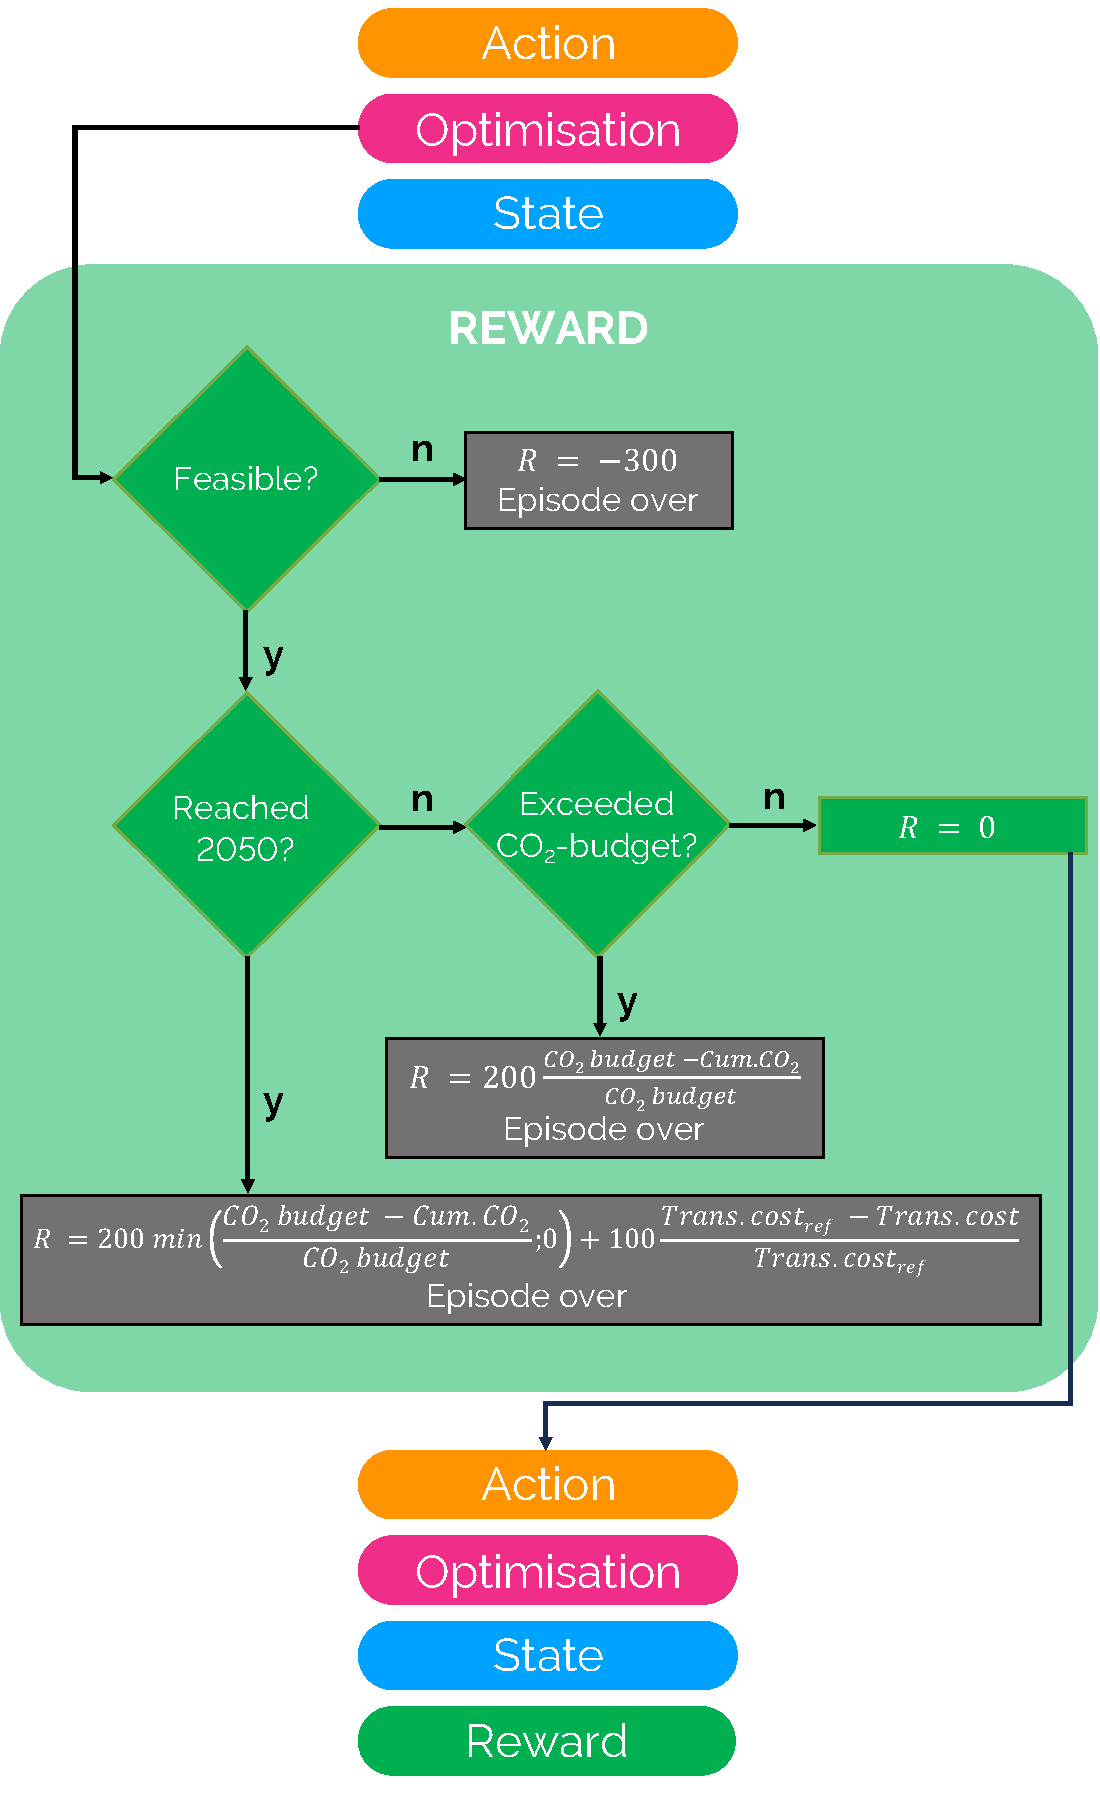
\includegraphics[width=0.65\textwidth]{Reward.pdf}
\caption{Reward function, $R$. Before reaching 2050, the episode is prematurely ended and a negative reward is given if the optimisation is infeasible or if the \ce{CO2}-budget is exceeded. If the optimisation provides a solution and the \ce{CO2}-budget is not exceeded, the episode continues. Finally, if the episode goes until 2050, the reward is a weighted sum between the capped cumulative emissions and the total transition cost.}
\label{fig:Reward}
\end{figure} 

First of all, taking a set of actions at a certain state might lead to an infeasible optimisation problem. In other words, as actions have a direct impact on some constraints of the problem, they might limit too much the feasible domain to the point where no solution can be found. For instance, the extreme case of aiming at carbon-neutrality, \ie $\mathrm{act}_{\mathrm{gwp}}=0$, and forbidding the use of the three aforementioned fossil fuels, \ie $\mathrm{act}\textsubscript{fossil gas}=\mathrm{act}\textsubscript{LFO}=\mathrm{act}\textsubscript{coal}=0$,  from the beginning of the transition makes the optimisation impossible to solve. In this case, the episode is prematurely ended and the reward is ``highly'' negative, -300. If EnergyScope is able to provide a solution to the time window to optimise and the end of the transition, \ie 2050, is not reached, a test on the cumulative emissions so far. On the one hand, if these cumulative emissions exceed the \ce{CO2}-budget, $1.2\,\text{Gt}_{\ce{CO2},\text{eq}}$ (see Section \ref{sec:cs:CO2-budget}), the episode is also ended and a penalisation is given to the agent. This penalisation is proportional to the difference between the \ce{CO2}-budget and the actual cumulative emissions.  On the other hand, the episode continues with a zero reward if the \ce{CO2}-budget is not exceeded. Eventually, if reaching 2050, we decided to tweak the reward function in capping the share of the cumulative emissions and integrating the transition cost. Given the main objective of the agent to respect the \ce{CO2}-budget and not to be more ambitious ``\ce{CO2}-ambitious'', we cut short the contribution of the cumulative emissions as soon as they are lower or equal to the \ce{CO2}-budget.  Moreover, to make the agent sensitive to the cost-impact of its policy, we added the total transition cost in the reward function where the \emph{Trans. cost$_{\text{ref}}$} on Figure \ref{fig:Reward} is equal to $1.1\cdot10^3$\,b€. This value comes from the mean of the total transition costs obtained through the \gls{GSA} performed on the perfect foresight transition pathway optimisation (see Section \ref{subsec:atom_mol:results_uq_cost}). In this final form of the reward, one will notice that overshooting cumulative emissions are more penalising than an overshooting transition cost, \ie weight of 200 for the emissions versus 100 for the cost. The values of these weights are the results of a trial and error. This way, we observed that the agent first targeted the respect of the \ce{CO2}-budget and then, to a lesser scale, avoided reaching over-costly transitions.\\

\myparagraph{States}\\

\noindent
Besides the reward, states are the other piece of information provided by the environment to the agent. In \gls{RL}, the purpose of states are to represent the current situation or configuration of the environment in which the agent operates. The primary function of states in RL is to provide the necessary context for the agent to choose appropriate actions based on its current observations and goals \cite{sutton2018reinforcement}. The challenge in the definition of the states is to provide enough information but not too much to avoid overwhelming the agent with non-informative features. 

Consequently, after another process of trial and error, we have converged to a four-dimension state space characterizing the energy system at the end of the optimised time window. The first dimension is directly related to the main objective of the agent: respecting the \ce{CO2}-budget until 2050. Therefore, the cumulative emissions emitted so far in the current step of the transition is the first dimension of the states. Similarly, the cumulative cost of the transition so far constitutes the second dimension of the states to inform the agent about the cost-impact of its actions on the environment. Finally, to enrich the level of details, we have added two other dimensions representative of the key-to-the-transition indicators identified by in Renewable Energy Directive (RED) III of the European Commission \cite{REDIII}: the share of renewables in the primary energy mix and, the energy efficiency. The former is computed as the share of local renewables (\ie wind, solar, hydro and biomass) and imported renewable energy carriers (\ie biofuels and electrofuels) in the total consumption of primary energy. Electricity imported from abroad is not considered in the set of renewable energy carriers even if it can be assumed to be fully renewable by 2050. Finally, even though energy efficiency is usually defined as the ratio between the \gls{FEC} and the primary energy mix, we decided to define this efficiency with a focus on the \gls{EUD}, like in the rest of this thesis. Where electricity, heat and non-energy \gls{EUD} are expressed in terms of energy content, we needed to convert passenger and freight transports into their respective \gls{FEC} to integrate them in the ratio. 

\section{Convergence and learning process}
\label{sec:RL:learning}

Before testing the optimal policy $\pi^*\left(\bm{a}_n | \bm{o}_n\right)$, the first step consists in assessing the learning of the \gls{NN}, also called ``training''. For this, numerous episodes are played through the myopic optimisation of the transition pathway of Belgium. At the beginning of each episode, the agent starts with the actual Belgian energy system of 2020 (see Appendix \ref{app:bel_2020}). Then, a sample of values, drawn for the uncertain parameters, affects the model for the 2020-2030 time window. This sample will remain valid for the following time windows. In other words, there is only one sample draw per episode (see Figure \ref{fig:ranges_transition}).  Then, the agent takes a set of actions, affecting the environment that feeds back the agent with a new state and a reward. This goes on until the end of the episode. For the new episode, similarly to the \gls{UQ} analysis (see Section \ref{sec:meth:UQ}), the new sample of uncertain parameters for the new episode is drawn following the quasi-random Sobol' sampling technique \cite{bratley2003implementing}.

To reduce the computational burden and maximise the exploration of the transition pathways, the learning phase of the agent has been done on the monthly model. Even though averaging time series of end-use demands and renewable productions brings some discrepancies (\ie faster emergence of local \gls{VRES} and smaller electrification of the system), the main advantage of the monthly approach is its computational time, \ie couple of seconds versus 15 min for the hourly model (see Appendix \ref{app:mo_vs_td}). \\

\myparagraph{Reward and success}\\

The learning phase has been split into batches of 500 steps. For the first 100 steps of each batch, the \gls{RL}-model collects transitions before learning starts. This makes sure replay buffer is full enough for useful updates. At the end of each batch, the up-to-date policy, \ie the \gls{NN}, is saved. This way, we can assess the progress in the learning process and its convergence (see Figure \ref{fig:reward_success}).  The mean reward increases rapidly at the beginning of the learning process before reaching a plateau where the optimisation of the policy becomes more marginal. Right hand side of Figure \ref{fig:reward_success} shows the success rate as the share of transitions meeting the \ce{CO2}-budget (see Section \ref{sec:cs:CO2-budget}) over the total number of attempted transitions, \ie episodes. Even though this success rate is not what drives the agent's optimisation, it shows that the shape of the reward (see Figure \ref{fig:Reward}) leads towards more and more successes. 

\begin{figure}[!htbp]
\centering
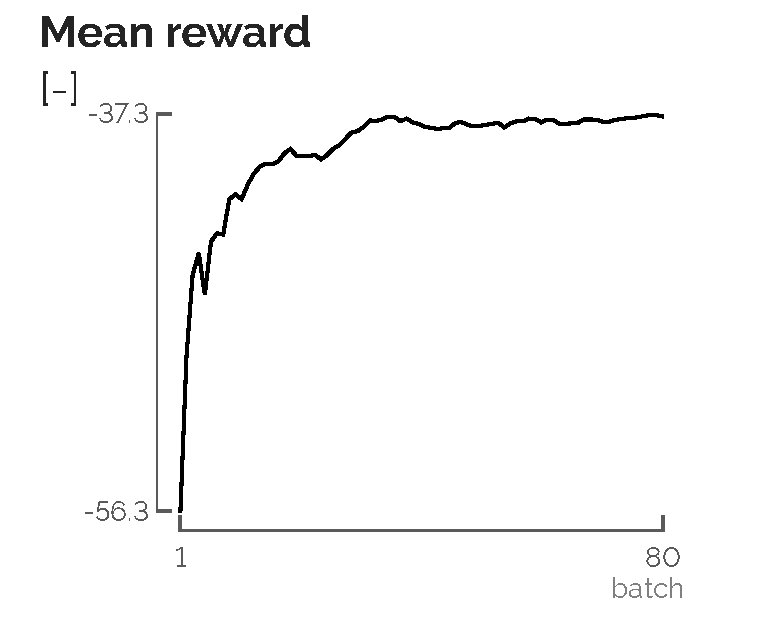
\includegraphics[width=0.49\textwidth]{Mean_reward.pdf}
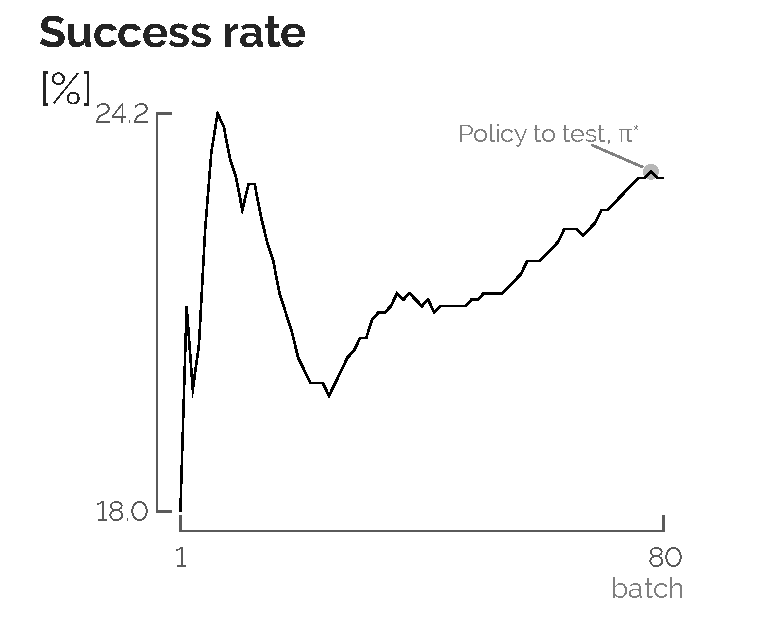
\includegraphics[width=0.49\textwidth]{Success_rate.pdf}
\caption{Mean reward and success rate of the different learning batches. The stabilisation of the reward curve shows a convergence of the learning process for the agent's point of view. The evolution of the success rate also shows the shape of the reward aims at more and more successful transitions.}
\label{fig:reward_success}
\end{figure}

During the learning process, the algorithm explores numerous transition pathways: 2037 successful transitions out of 10,751 attempts. Each pathway provides valuable insight into the best course of actions --- the primary goal of reinforcement learning. As a side benefit, the collection of all explored pathways also identifies the intermediate milestones to reach and the range of actions that must be avoided or must be taken. Yet, the exploration during this learning process is not exhaustive. The trends provided below are therefore not proven. The randomness of the process and the number of explored transition pathways still give us high confidence.

There is a range in the reward where failures and successes overlap (see Figure \ref{fig:reward_status}). This area corresponds to either transitions that exceed the \ce{CO2}-budget in 2050 but are cheaper than the total transition cost of reference (see Section \ref{sec:RL:act_states_rew}) or successful transitions that are more expensive. Besides this overlap, we observe that successes account for the majority of the cases where the reward is positive. This is another indication that the shape of the reward is appropriate in this exploration of successful transition pathways.

Considering the end of the time-window where the \ce{CO2}-budget is exceeded, the right hand side of Figure \ref{fig:reward_status} shows that 2040 is the ``tipping year'' for the agent. Beyond this point, through this learning process, the chances to succeed the transition were 38\%. In other words, mid-term actions are necessary to hope succeeding the transition.

\begin{figure}[!htbp]
\centering
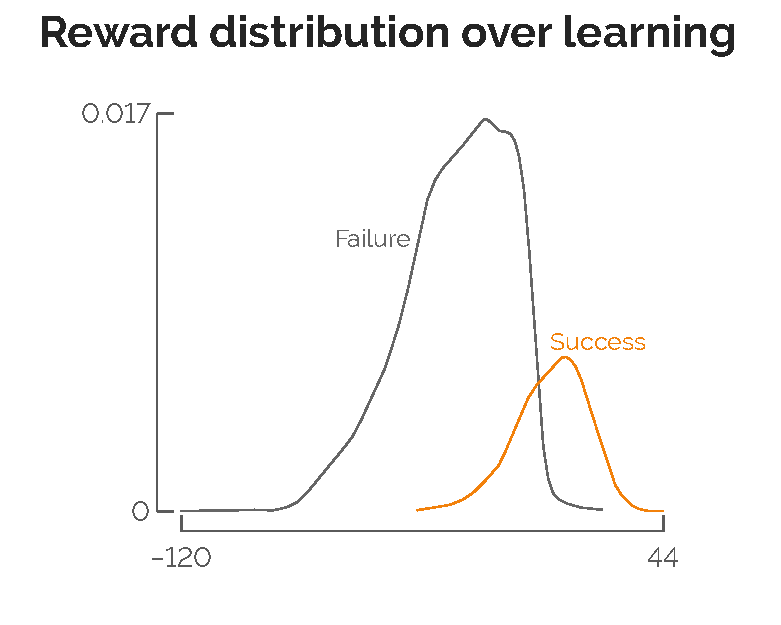
\includegraphics[width=0.49\textwidth]{Reward_status.pdf}
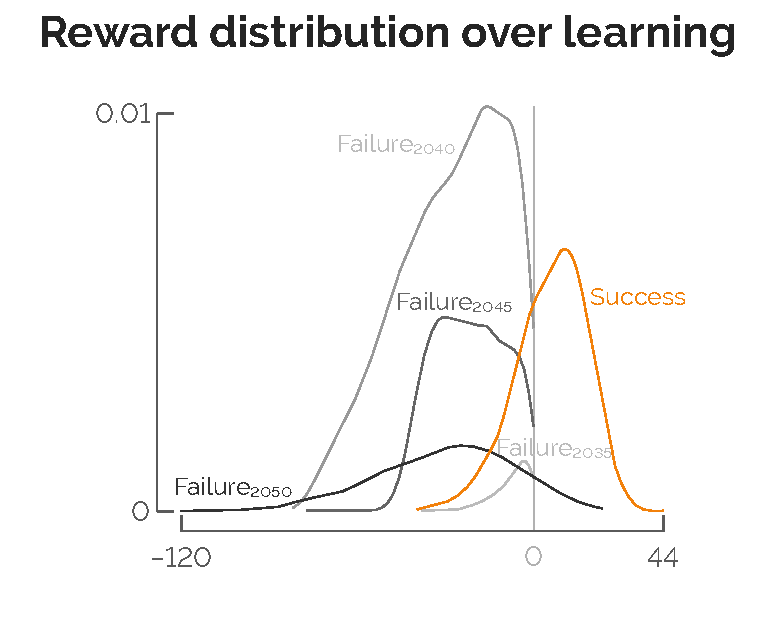
\includegraphics[width=0.49\textwidth]{Reward_status_2.pdf}
\caption{Reward distribution between successes and failures. Right hand side details at the end of which time-window the failure occurred. The ``tipping year'' is 2040 as failing the transition by 2040 represents 57\% of all the failures. Beyond this point, through this learning process, succeeding the transition represents 38\% of the episodes.}
\label{fig:reward_status}
\end{figure}

\myparagraph{States}\\

The first two dimensions of the state space are the cumulative emissions and costs. They drive the value of the reward and, consequently, the optimisation of the agent's policy. Per definition, the threshold of 1.2\,Gt\ce{CO2} splits the episodes reaching 2050 into successes and failures (see Figure \ref{fig:Cum_gwp_cost}). In the successful transitions, the median cumulative emissions, $\text{P}_{50}$,are about 0.9\,Gt\ce{CO2}. This is due to the combination of efforts made at earlier stages of the transition and the potential to install \gls{SMR} later on. Considering the failures, half of these episodes ended up with cumulative emissions lower or equal to 1.4\,Gt\ce{CO2}, 12\% higher than the \ce{CO2}-budget. As illustrated in Figure \ref{fig:reward_status}, 2040 is identified as the tipping year. Where 98\% of the failures were below the \ce{CO2}-budget in 2035, only 37\% passed this threshold in 2040. This reminds the importance of near-term actions to hope for a successful transition.

\begin{figure}[!htbp]
\centering
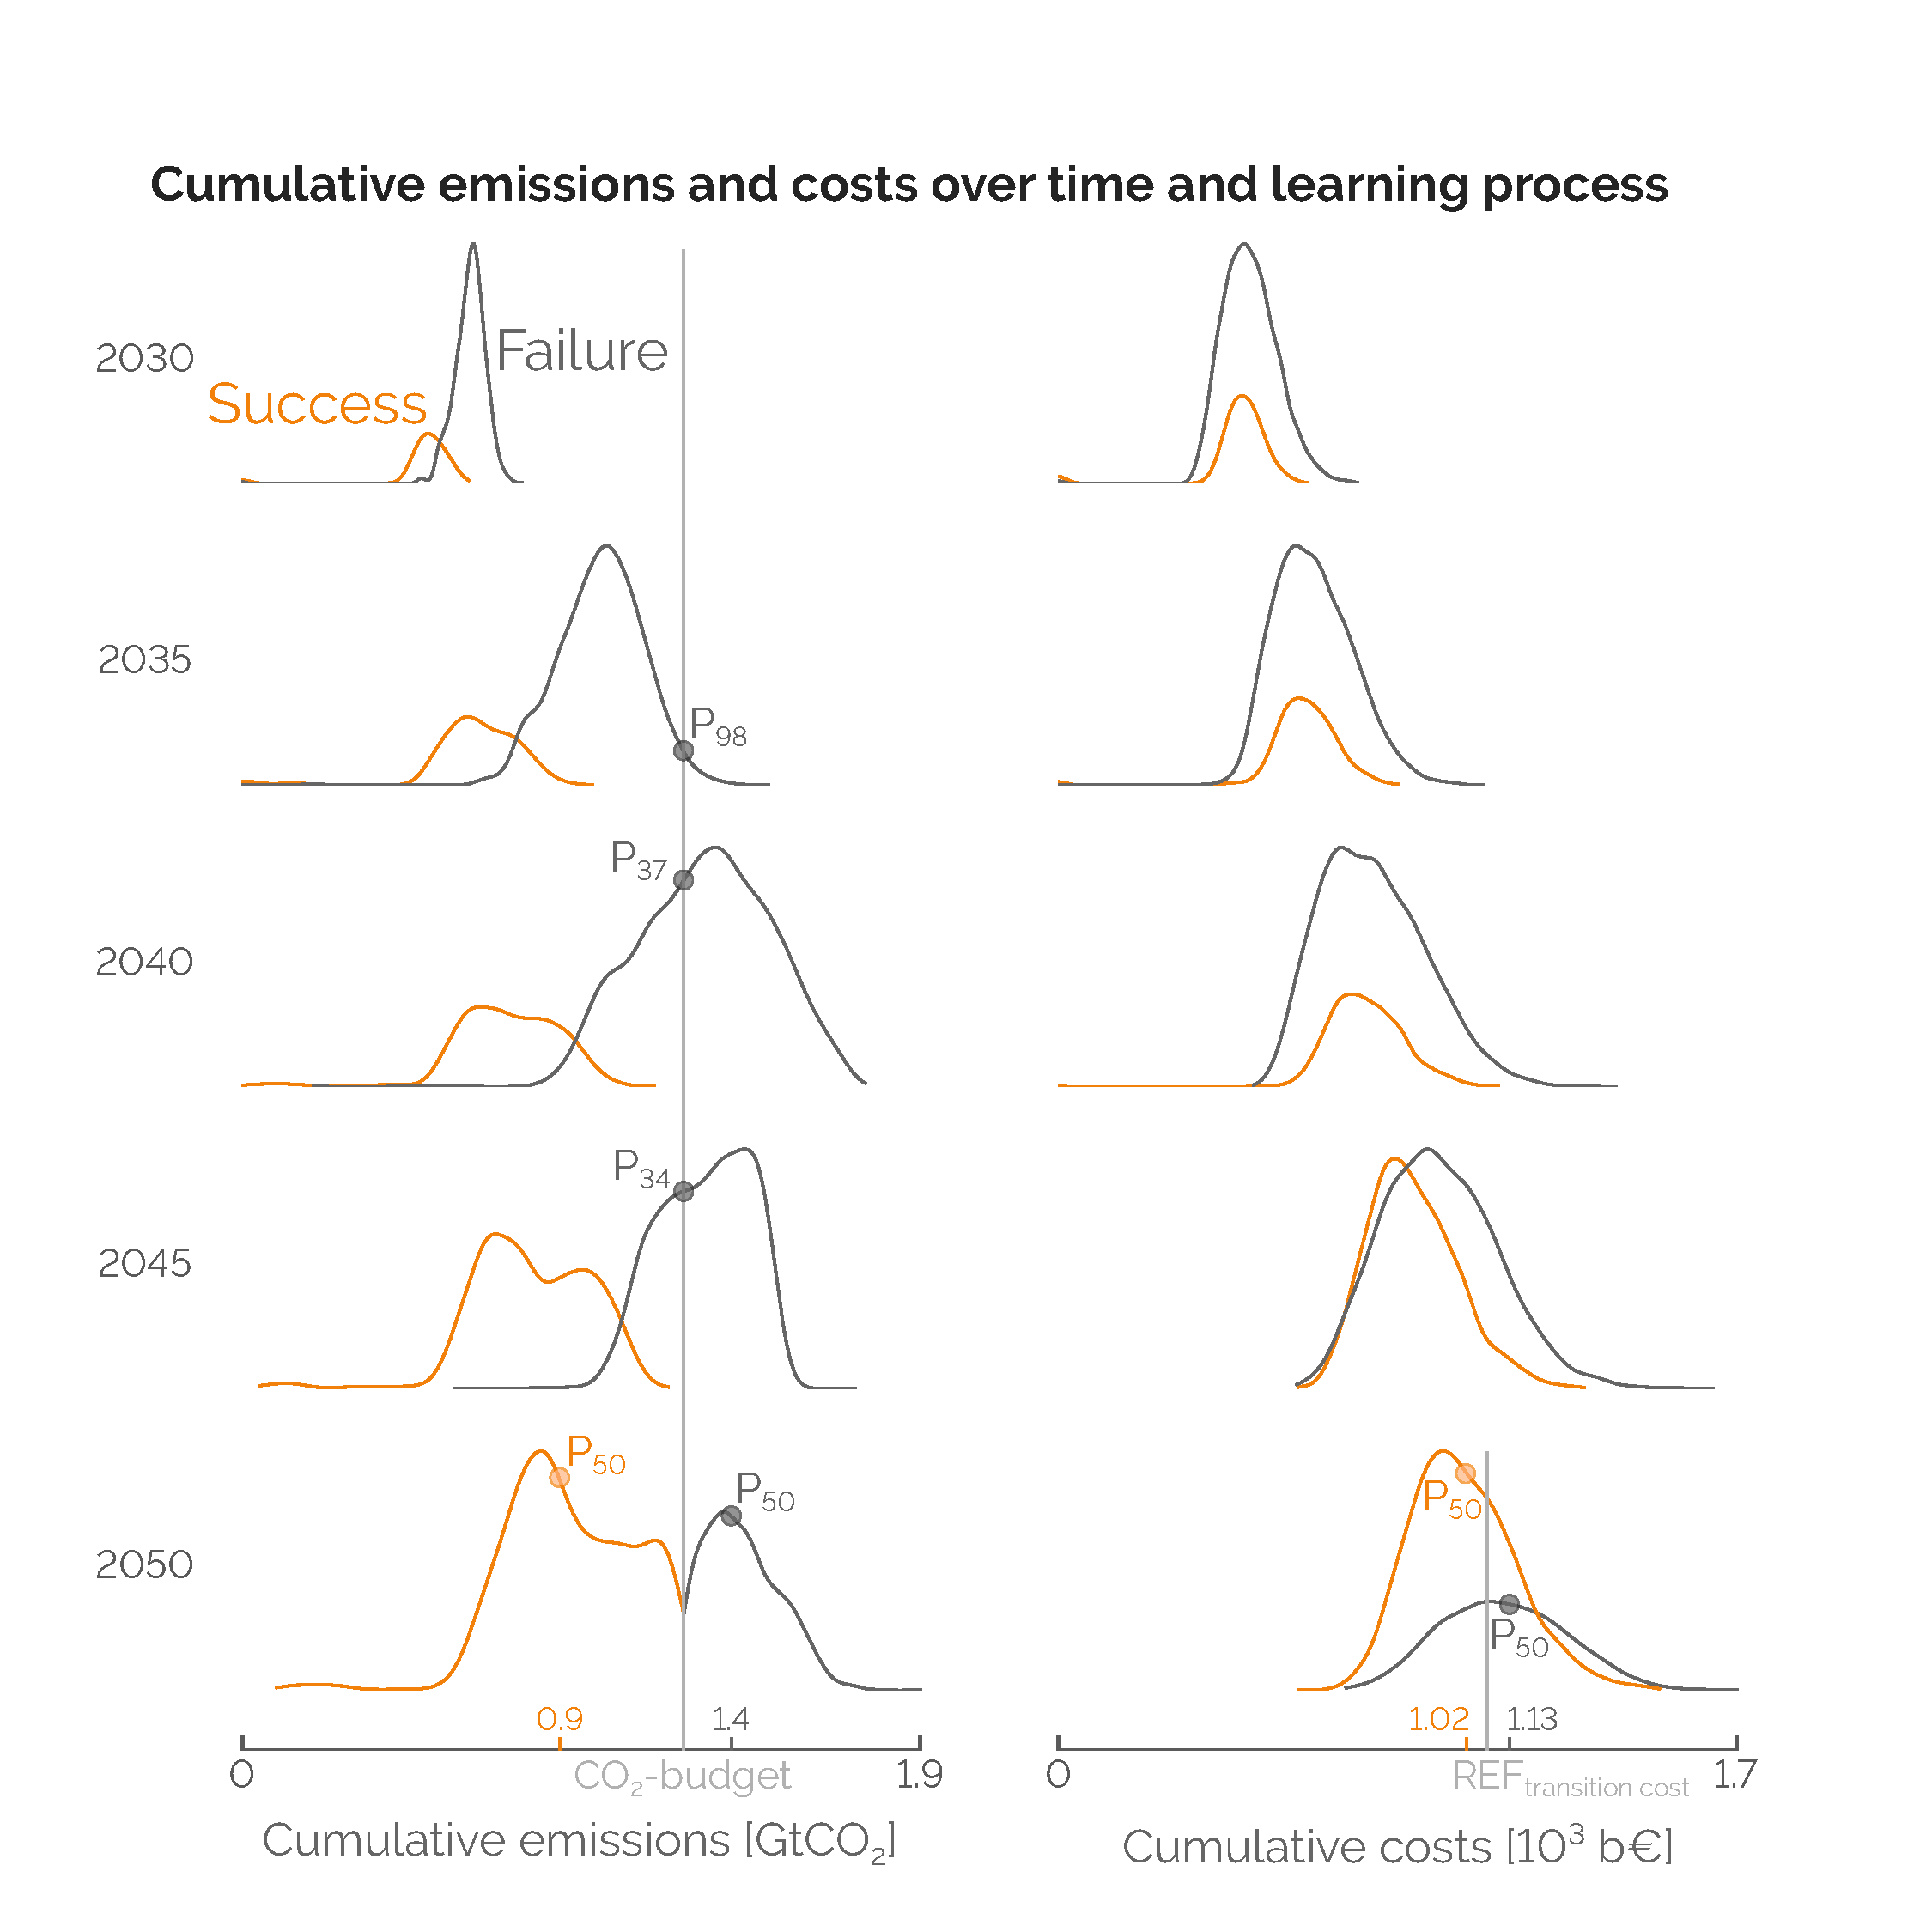
\includegraphics[width=0.8\textwidth]{Cum_gwp_cost.pdf}
\caption{Exploration of the state space over the learning process: cumulative emissions and costs. Successful transitions have cumulative emissions much lower than the \ce{CO2}-budget and are cheaper than the REF case. }
\label{fig:Cum_gwp_cost}
\end{figure}

Given the shape of the reward (see Figure \ref{fig:Reward}), the agent optimises its policy by aiming at lowering the total transition cost as soon as it meets the \ce{CO2}-budget. The skewness of the cumulative emissions and costs in 2050 are indications of this shape of reward (see Table \ref{tab:skewness_gwp_cost}). When succeeding the transitions, the cumulative emissions and costs have a negative and positive skewness, respectively. On the contrary, when it failed the transition, the agent aimed at reducing the emissions (skewness of 0.61) before minimising the total transition cost (skewness of 0.24). 

\begin{table}[htbp!]
\caption{Skewness of cumulative emissions and costs in 2050. Cumulative emissions are skewed to the left and to the right for the successes and failures, respectively. The skewness of the cumulative costs for successful transitions is higher compared to failures.On top of being the results of the optimisation through EnergyScope, these are influenced by the agent's policy that aims only at lowering the total transition cost as soon as it meets the \ce{CO2}-budget.}
\label{tab:skewness_gwp_cost}
\centering
\begin{tabular}{l c c}
\toprule
\textbf{Status of episode}  & \textbf{Skewness of cumulative} & \textbf{Skewness of cumulative} \\
\textbf{in 2050}  & \textbf{emissions} & \textbf{costs} \\	
\midrule
Success & -0.52 & 0.50 \\
Failure & 0.61 & 0.24 \\
\bottomrule							

\end{tabular}
\end{table}

Finally, we observe that the majority of the successful transitions are cheaper than the reference transition cost, 1.1\,b€. Among the parameters impacting the most the total transition cost, we observe that success occurs when, on average,  the cost of purchasing fossil fuels is more increased than the one of electrofuels (see Table \ref{tab:param_RL}).  Given the skewness that is positive and negative for the electrofuels and the fossil fuels, respectively, these cases represent more than the majority of the successful cases. On top of this, total transition costs of successful episodes are lower due to lower industrial \gls{EUD} and interest rate. These favourable conditions combined with the right agent's actions led to transitions respecting the \ce{CO2}-budget.

\begin{table}[htbp!]
\caption{Uncertain parameters impacting the most the total transition cost, their Sobol' index and, for the successful transitions, their mean of their values between 0 and 100\%, $\mu$, and their skewness, $\gamma$. On top of being supported by the agent's actions, successful transitions occur when the cost of purchasing fossil fuels is more increased than the one of electrofuels.}
\label{tab:param_RL}
\centering
\begin{tabular}{l c c c}
\toprule
\textbf{Parameter}  & \textbf{$\mu$} & \textbf{$\gamma$}  \\	
\midrule
Purchase electrofuels & 50.4\% & 0.004  \\
Industry EUD & 49.8\% & 0.026 \\
Interest rate & 48.4\% & 0.089\\
Purchase fossil fuels  & 55.0\% & -0.068\\
\bottomrule							

\end{tabular}
\end{table}

Besides the cumulative emissions and costs, the agent also observes the share of renewable energy carriers in the primary mix and the efficiency of the system The share of renewable energy carriers in the primary mix allows identifying intermediate milestones along successful transitions (see Figure \ref{fig:RE_in_mix_Efficiency}). From the initial state of 10\% in 2020, a boost of integration of renewables in the near-term is needed to hope for a successful transition. For the successful occurrences to exceed failures, this share increases to 54\% in 2025. Along the transitions, this increase goes with the import of electrofuels and the full deployment of local \gls{VRES}. In 2050, the success-failure threshold has been observed at 82\%. In the REF case of Chapter \ref{chap:atom_mol}, the share of renewables reached 86\% by 2050. However, by 2050, Figure \ref{fig:RE_in_mix_Efficiency} shows another threshold at lower share of renewables in the mix. This area corresponds to the possibility to install \gls{SMR}. As uranium is considered as a non-renewable resource \cite{rixhon2021terminology}, installing \gls{SMR} allows lowering the threshold to 60\% as in the SMR case of Chapter \ref{chap:atom_mol}. Besides these milestones to respect the \ce{CO2}-budget of the transition, one can also look at the other side of the thresholds. Below the near-term threshold of 60\%, this the ``no-go zone'' where succeeding the transition becomes unlikely, except if betting on the future installation of \gls{SMR}.

The efficiency, as defined in Section \ref{sec:RL:act_states_rew}, gives less valuable information to direct towards successful transition. Through the transition, besides the share of success increasing over the failures, these two scenarios indistinguishably spread over the whole range. Similarly than the emissions, we observe a bump at lower efficiencies by 2050 due to the installation of \gls{SMR}.

\begin{figure}[!htbp]
\centering
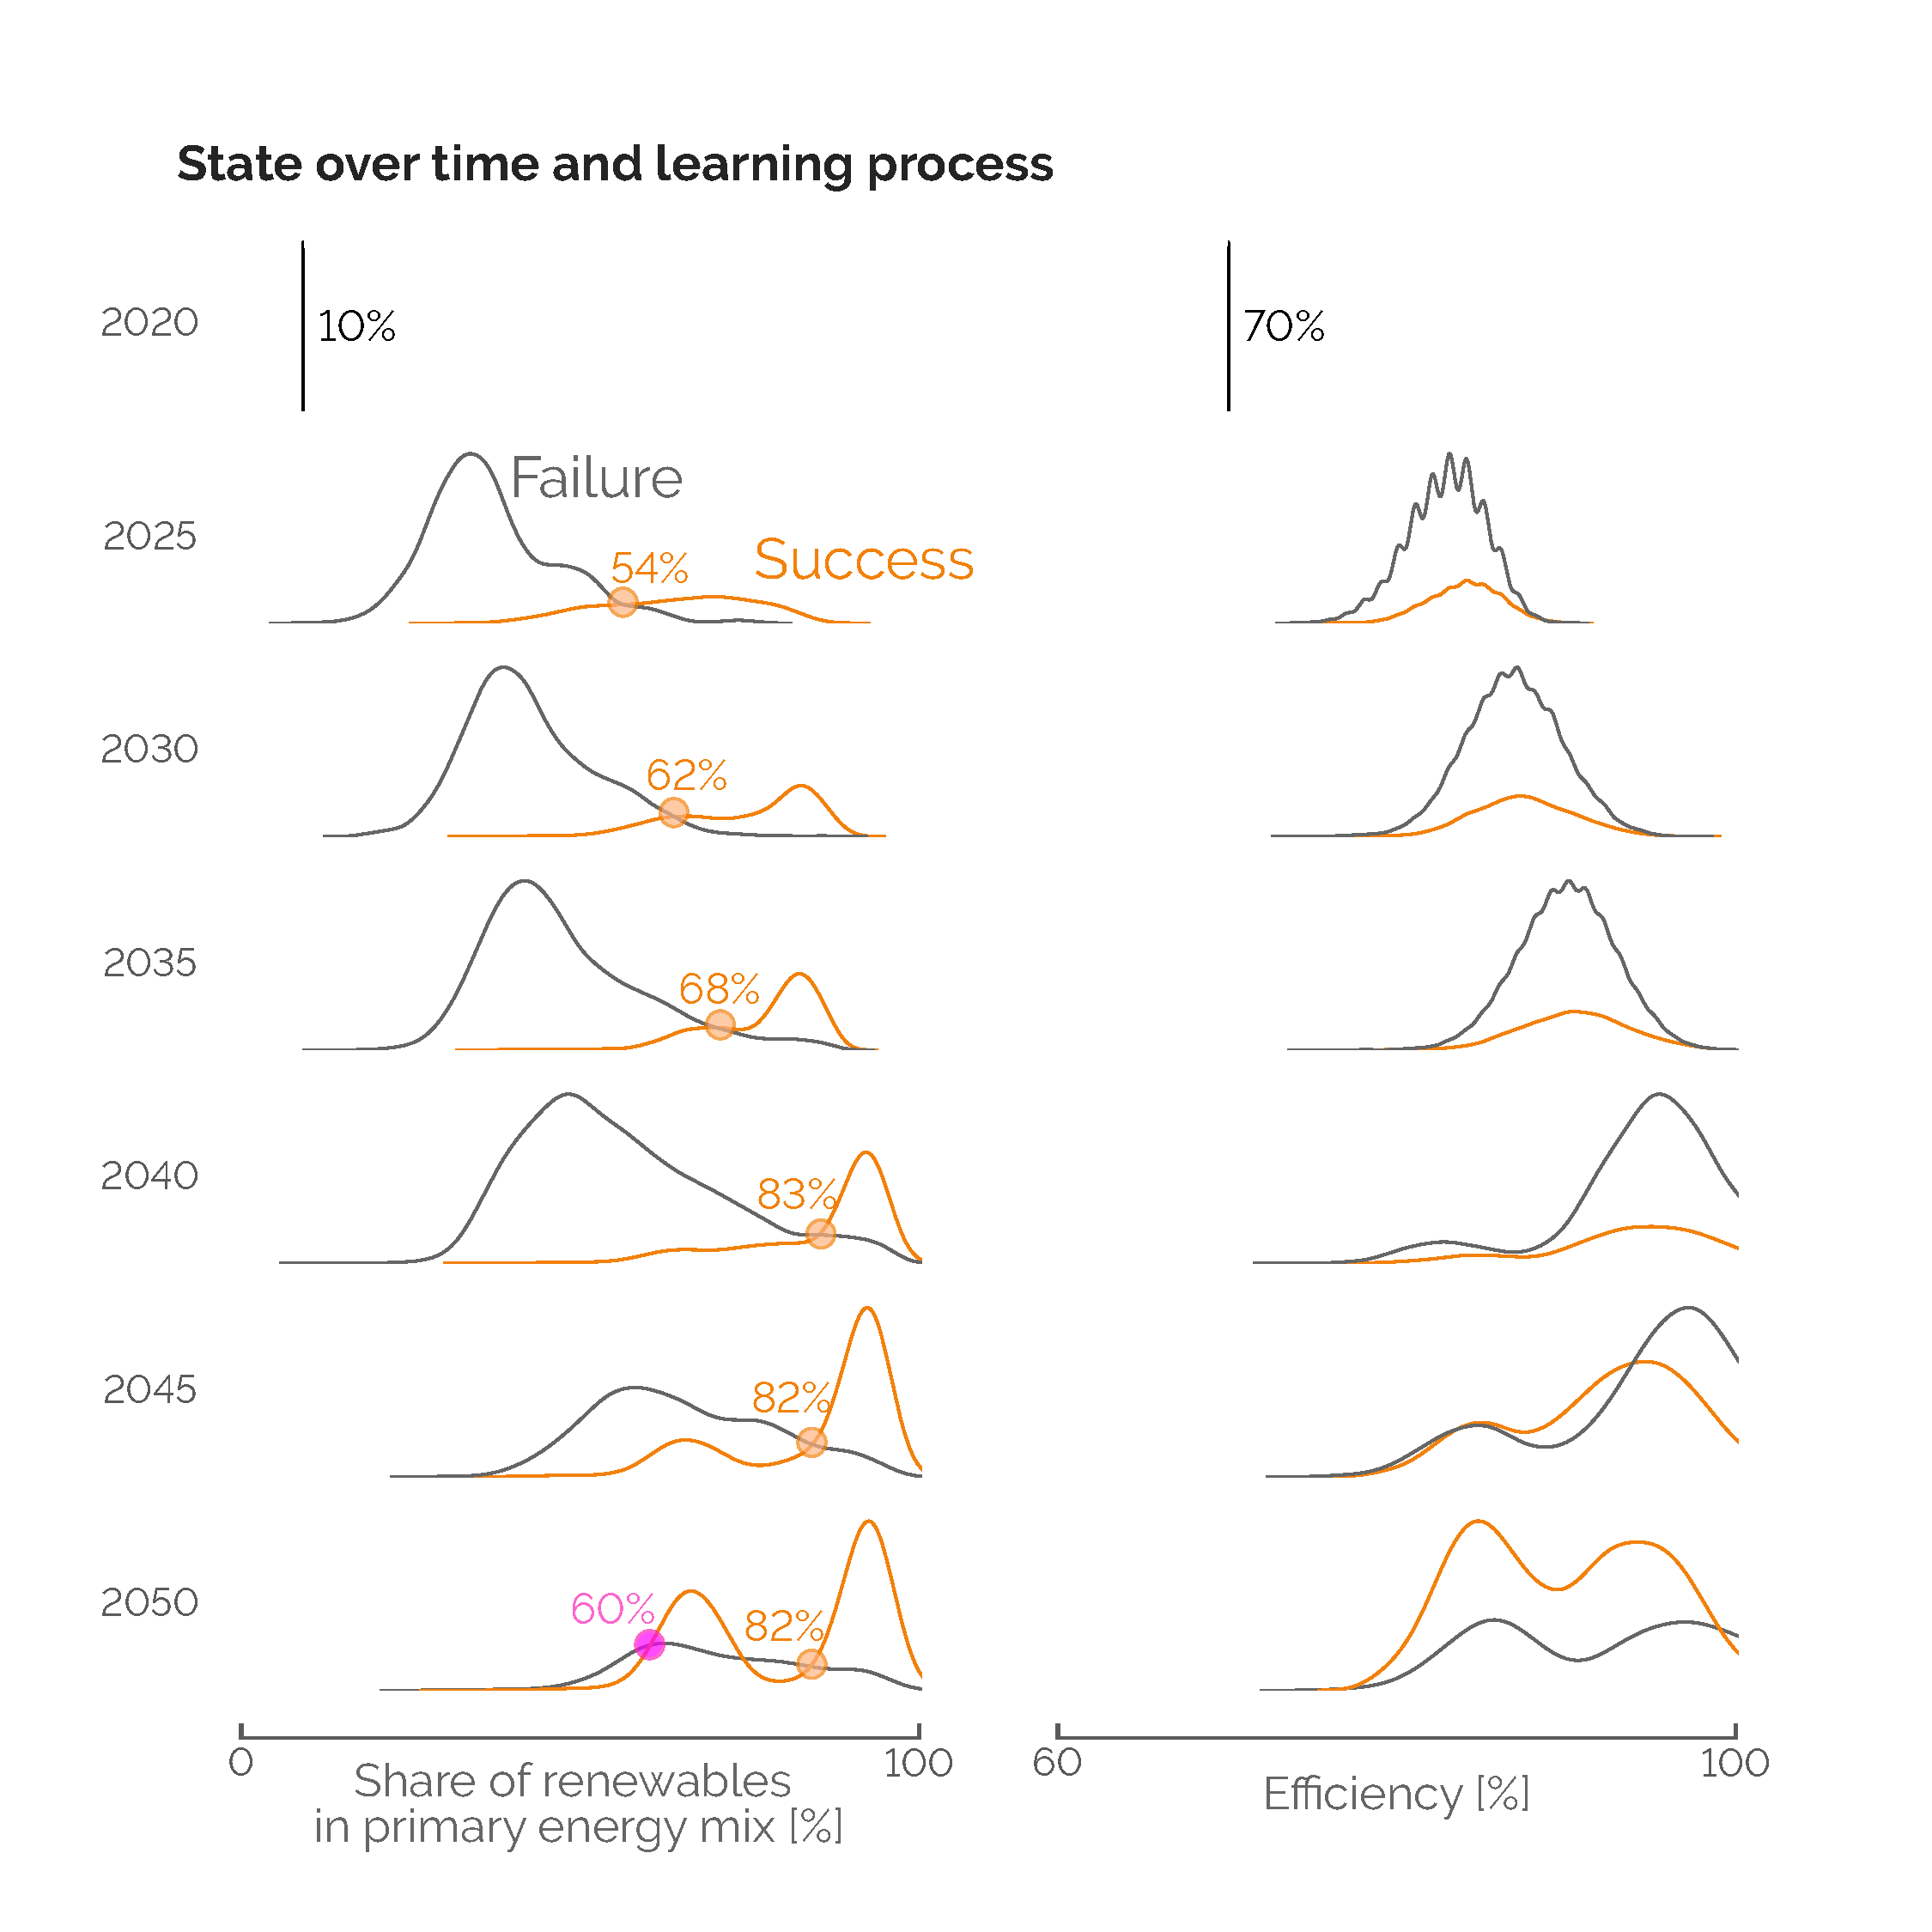
\includegraphics[width=0.8\textwidth]{RE_in_mix_Efficiency.pdf}
\caption{Exploration of the state space over the learning process: share of renewable energy carriers in the primary energy mix and efficiency. Integration of local \gls{VRES} at early stages then massive import of electrofuels later are needed to secure successful transitions. Below a near-term threshold (about 60\%), the chances of success are limited, \ie no-go zones. Efficiency is a less valuable information for the agent to succeed transitions as failures and successes indistinguishably spread over the whole range.}
\label{fig:RE_in_mix_Efficiency}
\end{figure}

\myparagraph{Actions}\\

After investigating the intermediate milestones to meet the \ce{CO2}-budget by 2050, this section details the actions the agent has taken during the learning process (see Figure \ref{fig:Actions_learning}). Rows represent the beginning of the time window at which the set of actions is taken. Similarly to the state space, we observe a wide exploration of the action space. The more the agent was able to progress through transition, without exceeding the \ce{CO2}-budget, the bigger is the share of successes compared to failures. Besides this observation, no specific range of values for the different actions at the different timing seems to lead to more successes. In other words, there is no clear set of actions that would support more effectively the transition.

\begin{figure}[!htbp]
\centering
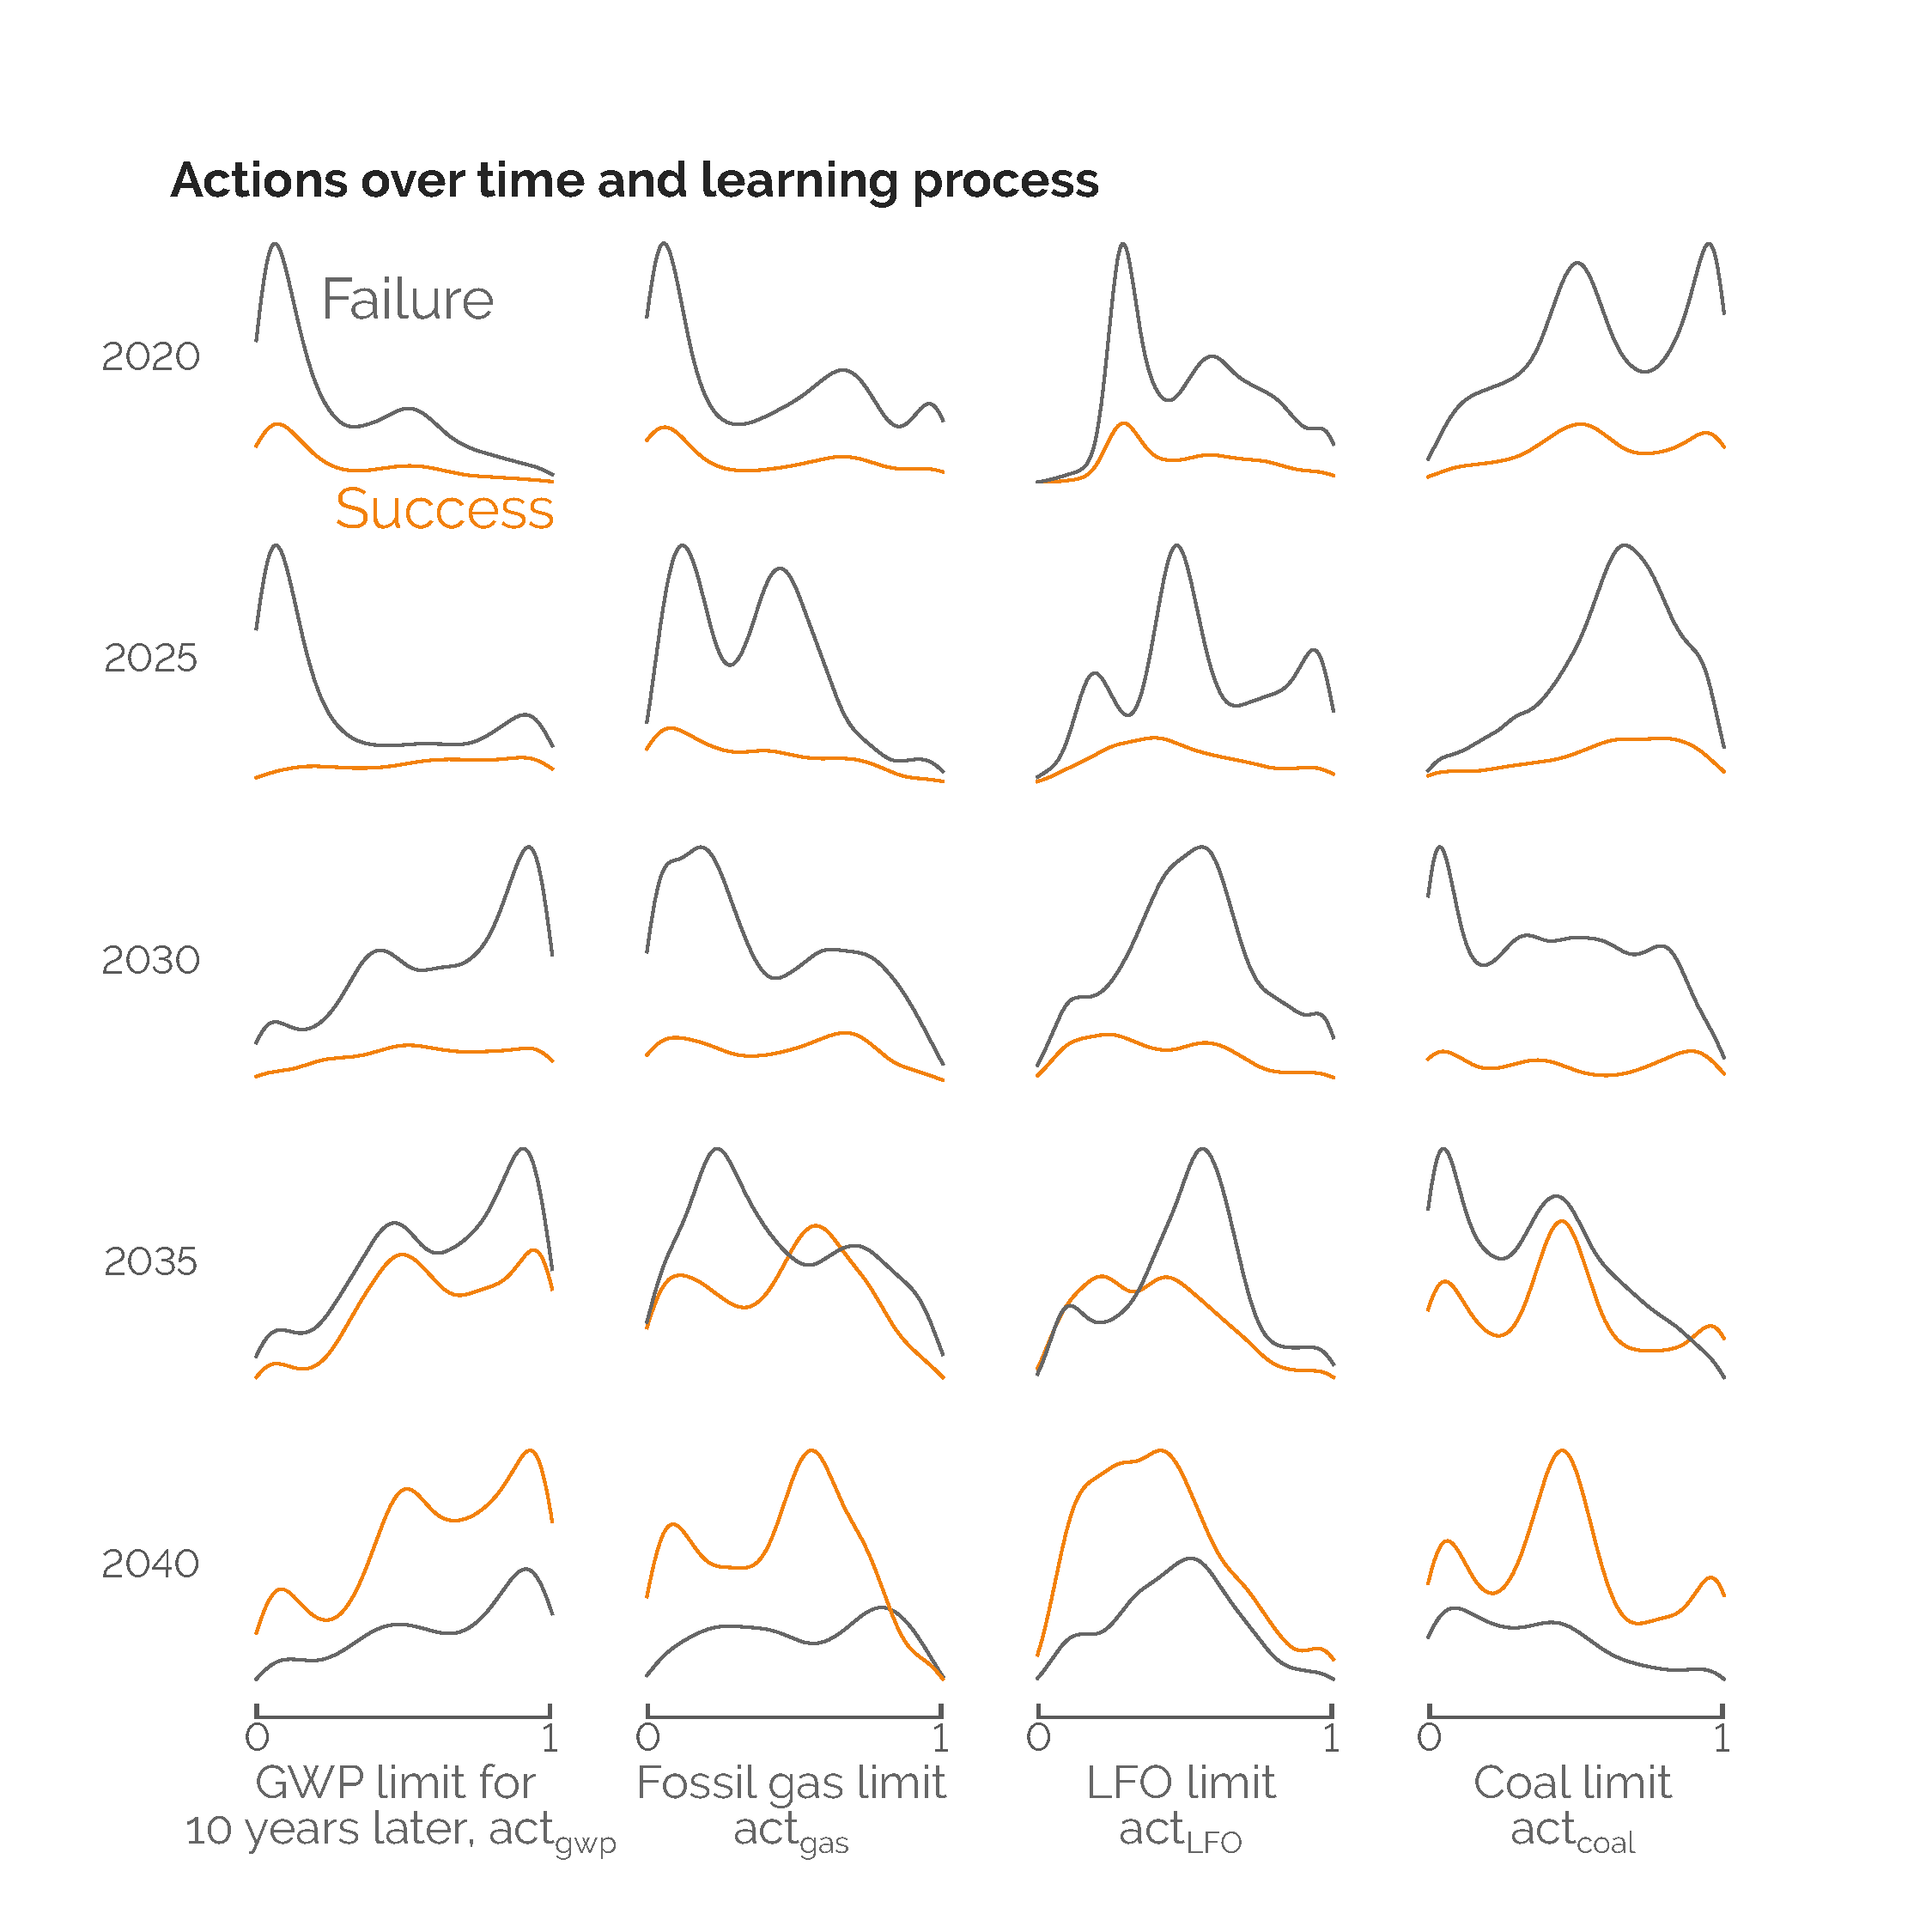
\includegraphics[width=0.8\textwidth]{Actions_learning.pdf}
\caption{Besides the wide exploration of the action space, successes and failures indistinguishably spread over the whole ranges of actions. In other words, it does not seem to be any clear set of actions to support successful transitions.}
\label{fig:Actions_learning}
\end{figure}

To identify the actions that have an actual impact on the environment, we can check if they were binding or not. In a \gls{LP} problem, constraints represent hyperplanes in the domain of variables. In a two-dimension space, these are straight lines (see Figure \ref{fig:Binding_constr}). When the problem is bounded and feasible, these lines are the edges of a convex polygon, the domain of feasibility. The optimal solution, $\textbf{x}^*$, is the combination of variables leading to the optimal value of the objective function. Besides being within the domain of feasibility, it is proven that this optimal solution, when unique\footnote{There are cases where the objective function has the same optimal value along an entire edge. In this case, there is an infinity of solutions and the problem is indeterminate.}, locates on a vertex of the domain \cite{bertsimas1997introduction}. The constraints intersecting at this vertex are considered as binding, actually limiting the objective function to be more optimal. In other words, binding constraints, when tightened, aggravate the objective value function. If these are inequality constraints, as represented in Figure \ref{fig:Binding_constr}, it means that their left and right sides of the equation are equal.

\begin{figure}[!htbp]
\centering
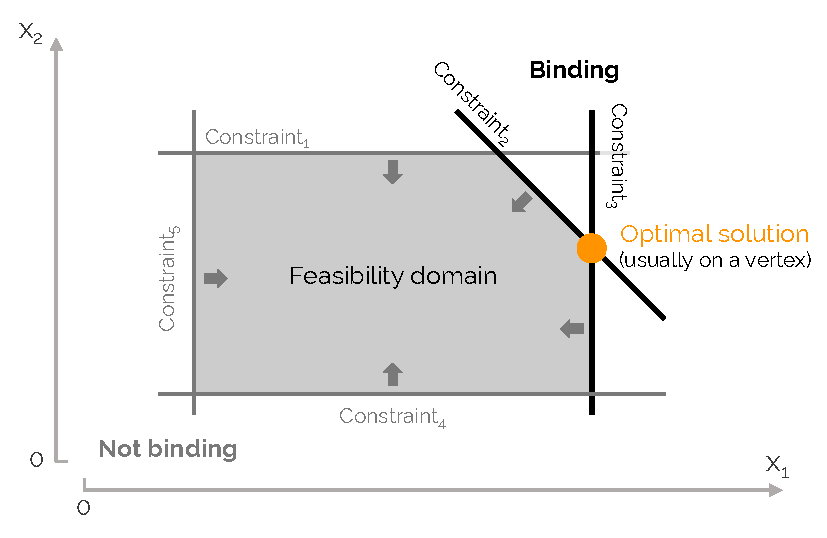
\includegraphics[width=0.7\textwidth]{Binding_constr.pdf}
\caption{Binding versus non-binding constraints. In \gls{LP} where the feasibility domain is non-empty and bounded, the constraints defined a convex feasibility domain in the space of variables (here, x$_1$ and x$_2$). The optimal solution usually locates on a vertex of this domain, \ie the intersection of several constraints (here, constraints 2 and 3) limiting the solution. These constraints are considered as binding, \ie having a limiting impact on the optimal solution.}
\label{fig:Binding_constr}
\end{figure} 

After filtering out failures of the learning episodes and keeping only the successful transitions, only a limited set of the actions are binding and have an actual impact on the result of the optimisation in EnergyScope Pathway (see Figure \ref{fig:Binding_learning}). This allows identifying key actions to support the myopic transition.Limiting the \gls{GWP} in the near-term is a key-factor for success. However, this action has an effective impact on the environment only when it forces the system to be close to carbon-neutrality. The range over which limiting the use of fossil gas binds the optimisation is wider. Compared to other non-renewable fuels, this is due to the longer use of this energy carrier favoured by its low \gls{GWP} (the second after uranium) and its versatility (applications in the electricity, heat and mobility sectors).

When it comes to limiting the use of \gls{LFO} and coal, the conclusions are more straightforward. At the beginning of the transition, most of the 159TWh of \gls{LFO} are consumed by naphtha-cracker (46\%) and decentralised boilers (45\%). The remaining 10\% are consumed by industrial boilers. Even though \gls{LFO} represents  30\% of the primary energy mix in 2020, the cost-optimum removes it of the mix without requiring the action of the agent. Naphtha-crackers, decentralised and industrial boilers get substituted by \gls{MTO}, decentralised \gls{HP} and industrial resistors and \gls{CHP}, respectively.  This ``non-bindness'' of limiting \gls{LFO} is an indication that this action could be removed from the agent's levers of action without impacting the optimisation of its policy.

On the contrary, limiting coal is always binding. Before all, this is due because coal is a cheap resource (17€/MWh). In other words, the cost-driven environment will favour it. Then, as the maximum amount of coal (28\,TWh) is much smaller than fossil gas and \gls{LFO}, high value of $\mathrm{act}\textsubscript{coal}$ still represents small consumption of coal.

\begin{figure}[!htbp]
\centering
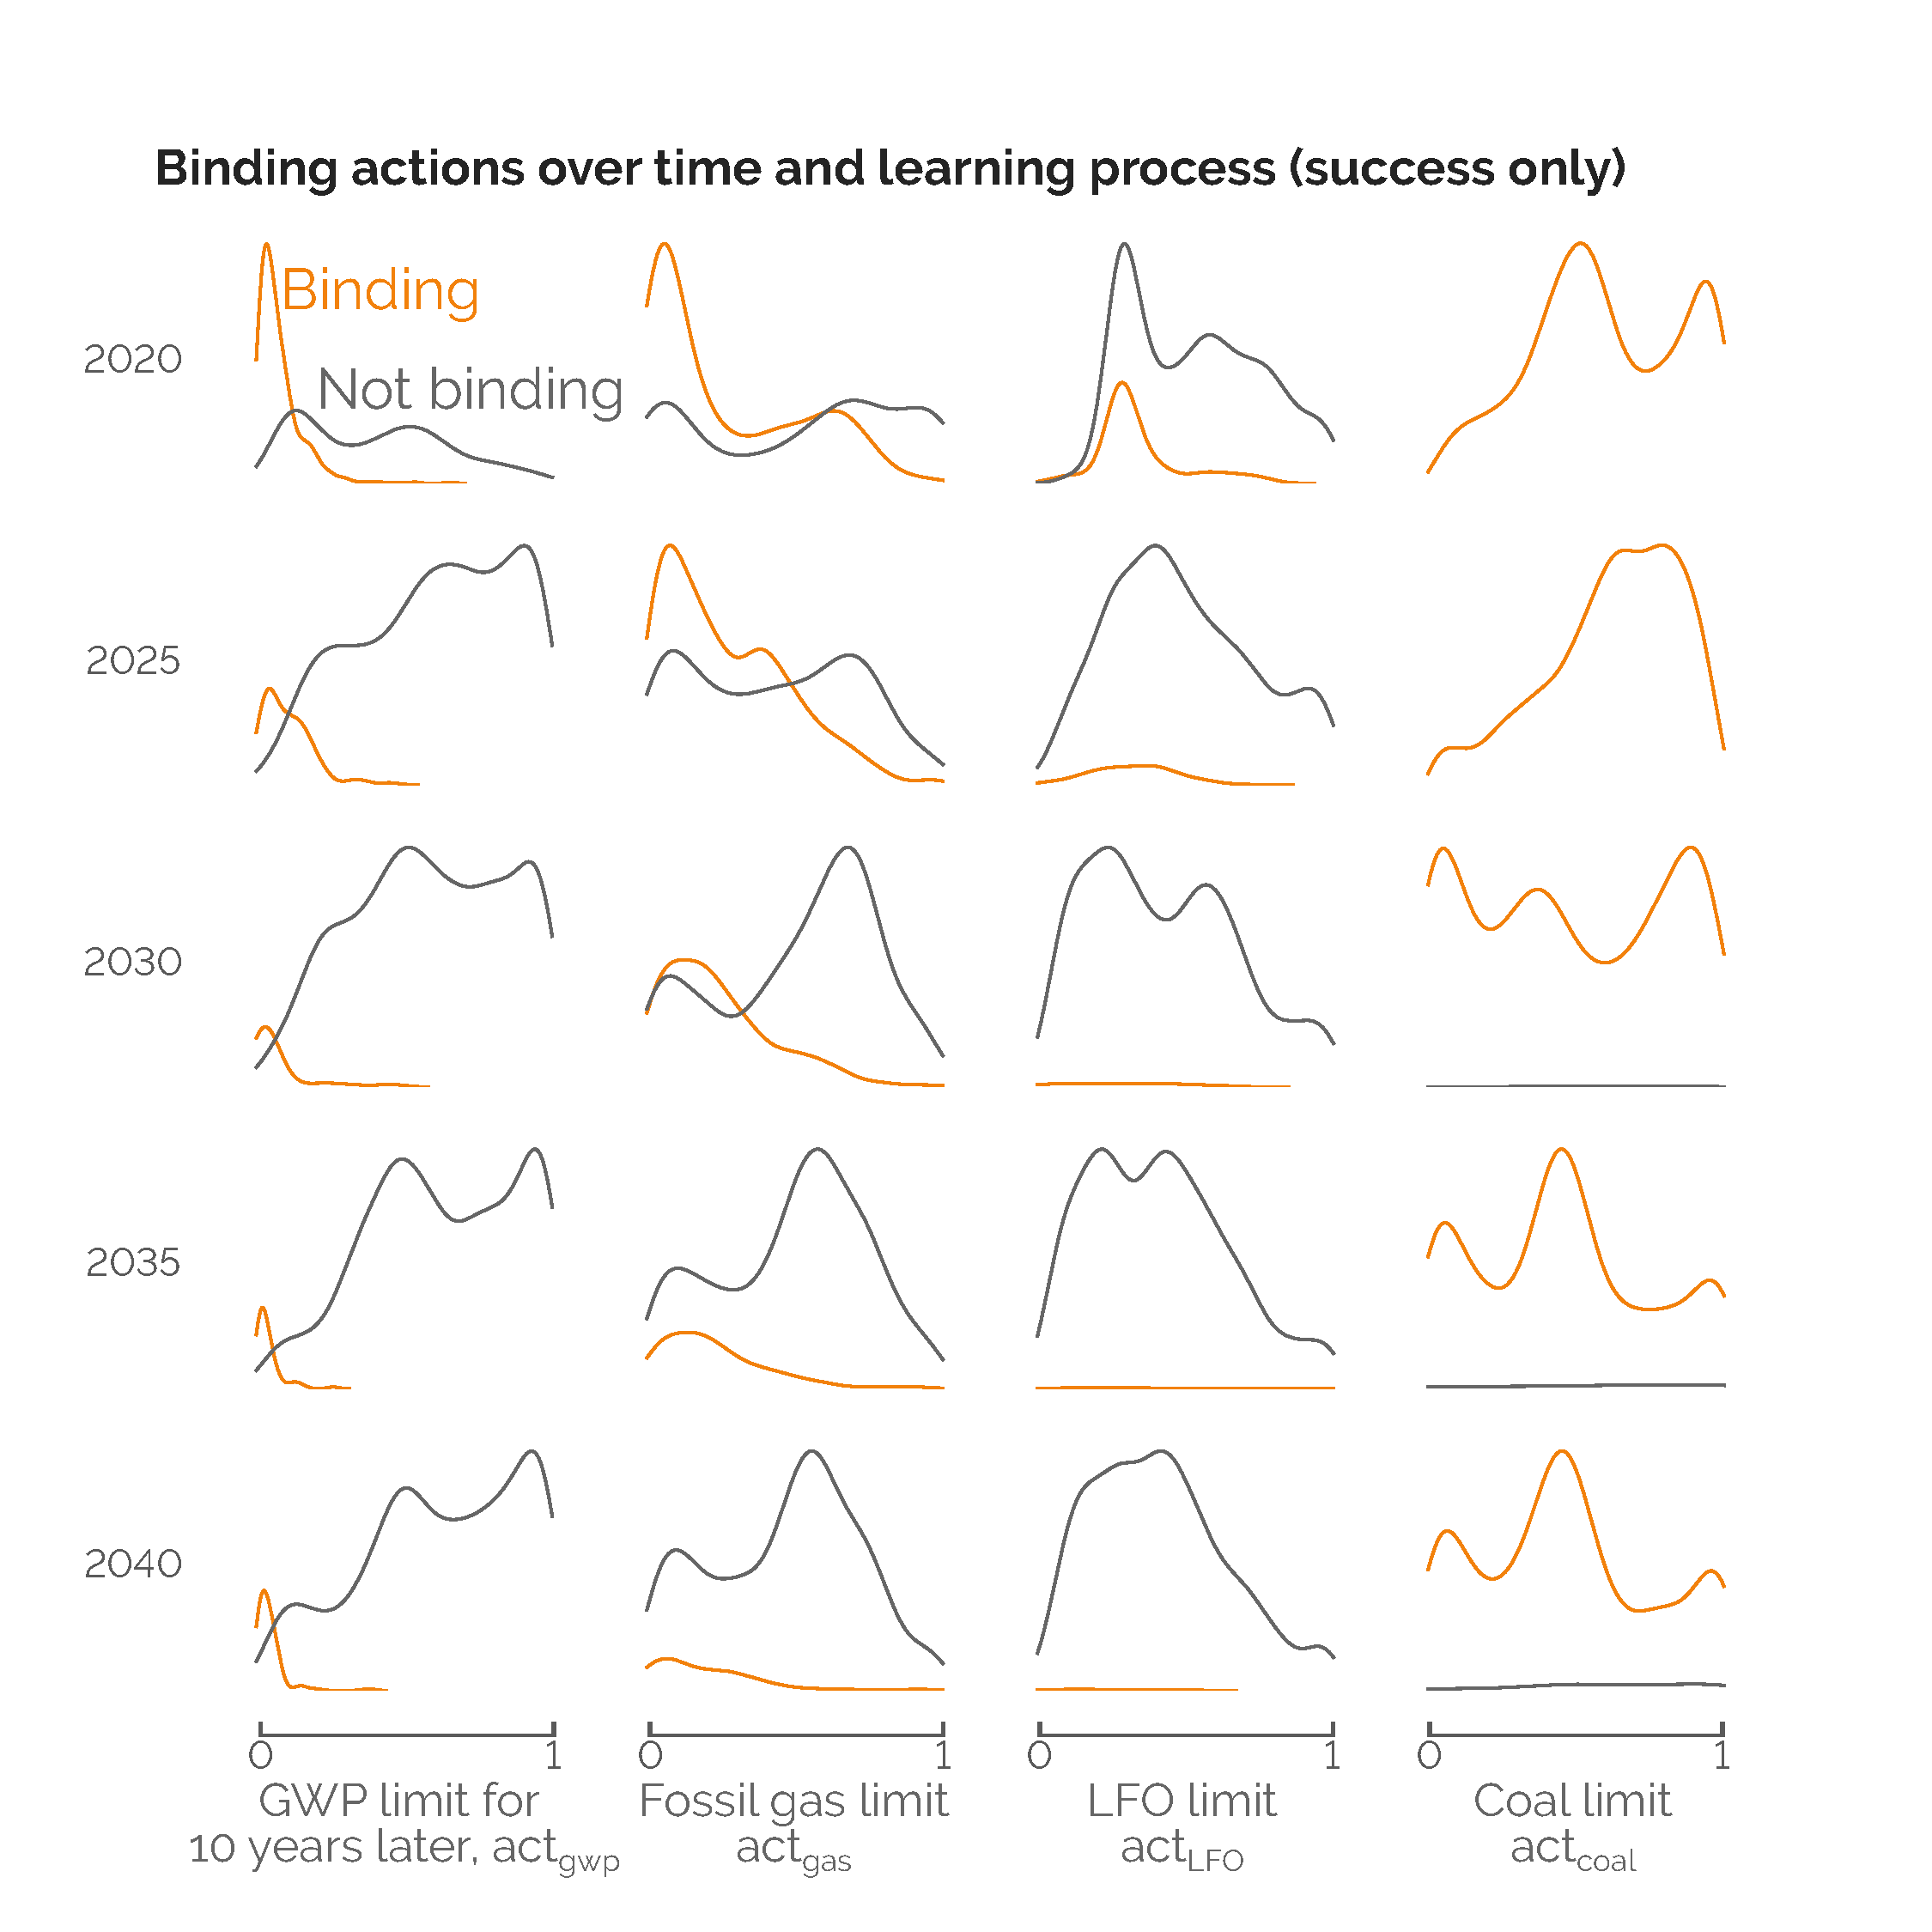
\includegraphics[width=0.8\textwidth]{Binding_learning.pdf}
\caption{Depending on the action and its timing, it is actually constraining the optimisation through EnergyScope Pathway or not. Sweet spots can be identified when considering the limits of \gls{GWP} and fossil gas consumption. Limiting coal consumption is always constraining, unlike \gls{LFO} that is ``naturally'' substituted by EnergyScope Pathway in the near-term.}
\label{fig:Binding_learning}
\end{figure}

\section{Comparison with references}
\label{sec:RL:testing}
After investigating the exploration of transition pathways on the monthly model, this section compares these results with two references: the \gls{RL}-agent trained on the hourly model and the perfect foresight under uncertainties from the \gls{UQ} analysis presented in Chapter \ref{chap:atom_mol}. The first reference has been built by applying the same rules (see Section \ref{sec:RL:act_states_rew}) but on the hourly model over a more limited number of batches, 43 versus 80, leading to 928 versus 2037 successful transitions for the results presented in Section \ref{sec:RL:learning}. First, the purpose is to assess the capacity of the monthly model to be a good proxy of the hourly myopic transitions and, then,  compare the explored pathways with the perfect foresight under uncertainties.

Considering the actions taken by the agent and their binding effect on the environment,  we see similar trends as in the monthly model (see Figure \ref{fig:Binding_learning_TD}). Limiting the consumption of coal is always binding where \gls{LFO} is ``naturally'' removed from the mix by the cost-minimisation. Where limiting the consumption of fossil gas has a major impact at the early stages, limiting the system emissions up to carbon-neutrality becomes more crucial at the end of the transition.

\begin{figure}[!htbp]
\centering
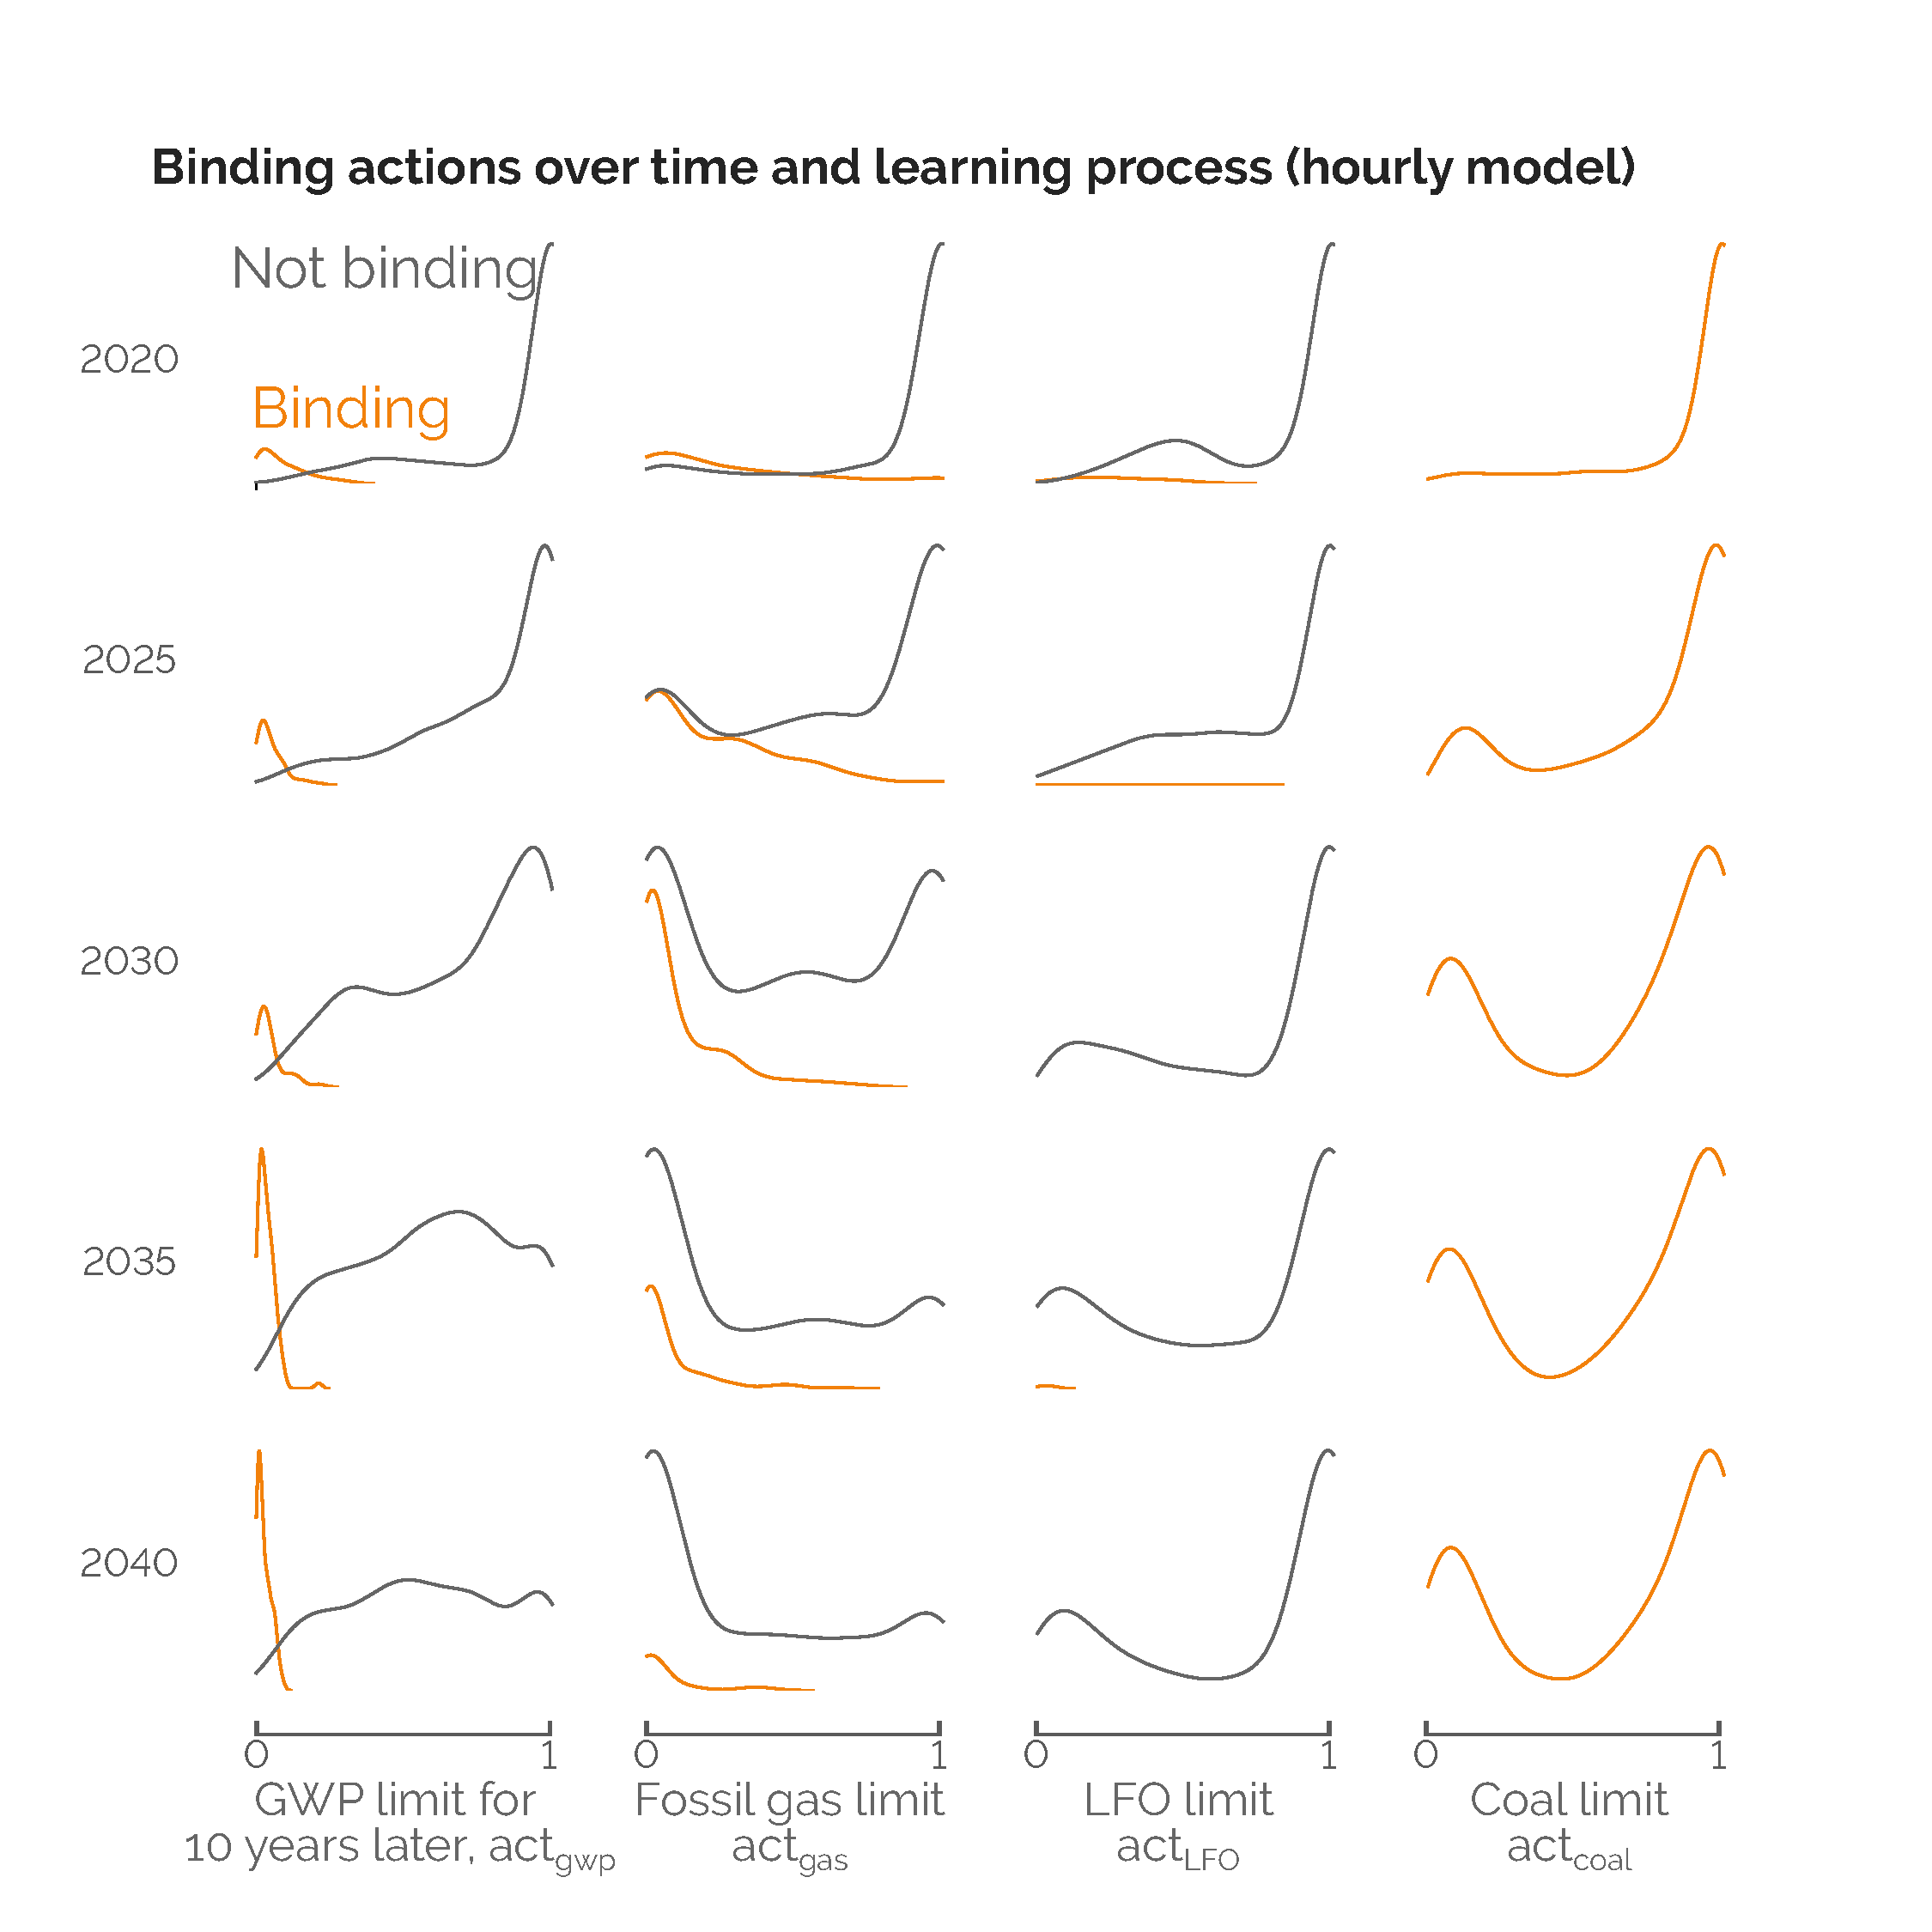
\includegraphics[width=0.8\textwidth]{Binding_learning_TD.pdf}
\caption{When the agent learns on the hourly model, the actions are binding in the similar timing and similar ranges as when learning on the monthly model. }
\label{fig:Binding_learning_TD}
\end{figure}

\gls{RL}-based myopic optimisation provides \ce{CO2}-emissions pathways different from the perfect foresight approach to respect the same \ce{CO2}-budget (see Figure \ref{fig:Gwp_pathway}). However, driven first by this \ce{CO2}-budget, the agent often reaches much lower cumulative emissions when succeeding the transition (see Figure \ref{fig:Cum_gwp_cost}). This comes from the agent's actions that limit the emissions and/or the consumption of fossil resources at the early stages. Thanks to the bigger reduction of emissions at these early stages, the \gls{RL}-based optimisation can benefit from a ``\ce{CO2}-buffer'' at the end of the transition. This buffer is compensated by the end of the transition where the 50\% of the myopic transitions reach 2050 with 9 or more Mt\ce{CO2} compared to 4 for the perfect foresight approach. These remaining emissions by 2050 come from the consumption in industrial boilers of waste and coal that account for 3.5\% and 2.4\% on average by 2050. The difference in the early drop of emissions between the monthly and hourly models comes from the easier integration of local \gls{VRES} as the hourly intermittency is averaged over a month (see Appendix \ref{app:mo_vs_td}). Besides this sharper decrease of emissions early in the transition, the monthly myopic pathways fit with the trend provided by \gls{RL} optimisation on the hourly model. Finally, the long-term vision of the perfect foresight approach results in smoother reduction of the emissions to end up with less emissions by 2050.

\begin{figure}[!htbp]
\centering
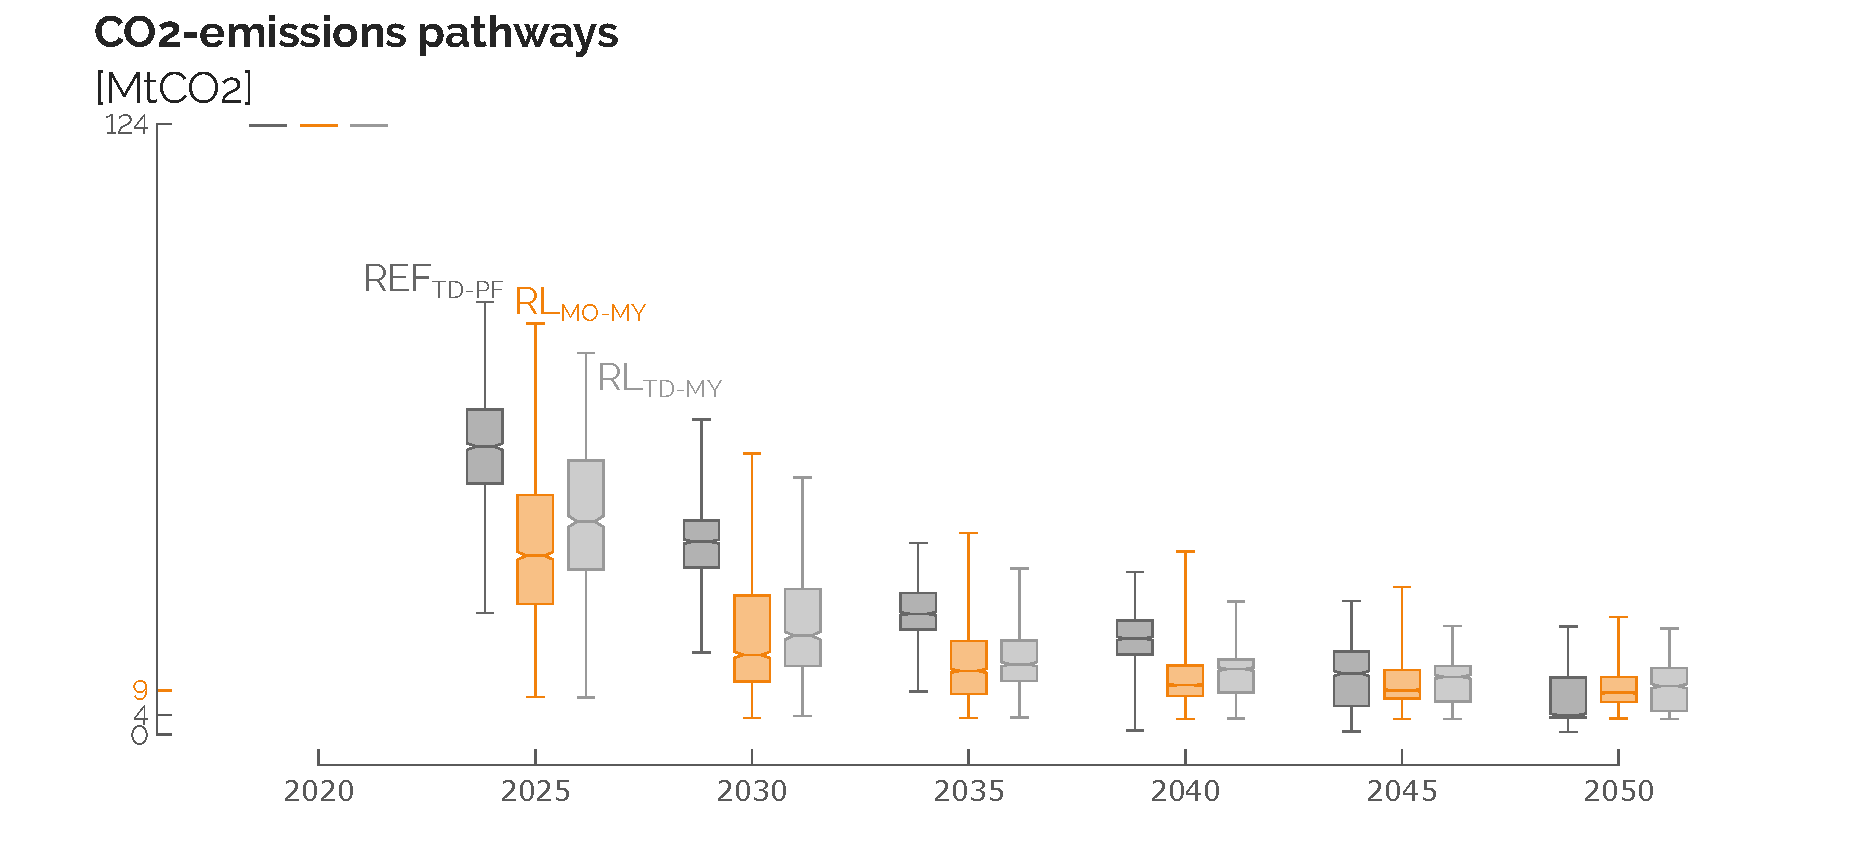
\includegraphics[width=0.8\textwidth]{Gwp_pathway.pdf}
\caption{Comparison of \ce{CO2}-emissions pathways from the perfect foresight optimisation under uncertainties ($\text{REF}_{\text{TD-PF}}$), the \gls{RL}-based myopic optimisation on the monthly ($\text{RL}_{\text{MO-MY}}$) and hourly ($\text{RL}_{\text{TD-MY}}$) models.}
\label{fig:Gwp_pathway}
\end{figure}

The transition pathways of the annual system cost also show the advantage of the \gls{RL}-based exploration (see Figure \ref{fig:System_cost_pathway}). Via its actions and its cost-based reward, the agent can reach systems that are cheaper than any other solution obtained by the perfect foresight approach. Even more than for the emissions, the monthly model is a good proxy to assess the annual system cost of the pathway on the hourly model. The perfect foresight approach gives a wider variability in its cost since this method always found a solution even in worst conditions such as high cost of purchasing resources and high \gls{EUD}. 

\begin{figure}[!htbp]
\centering
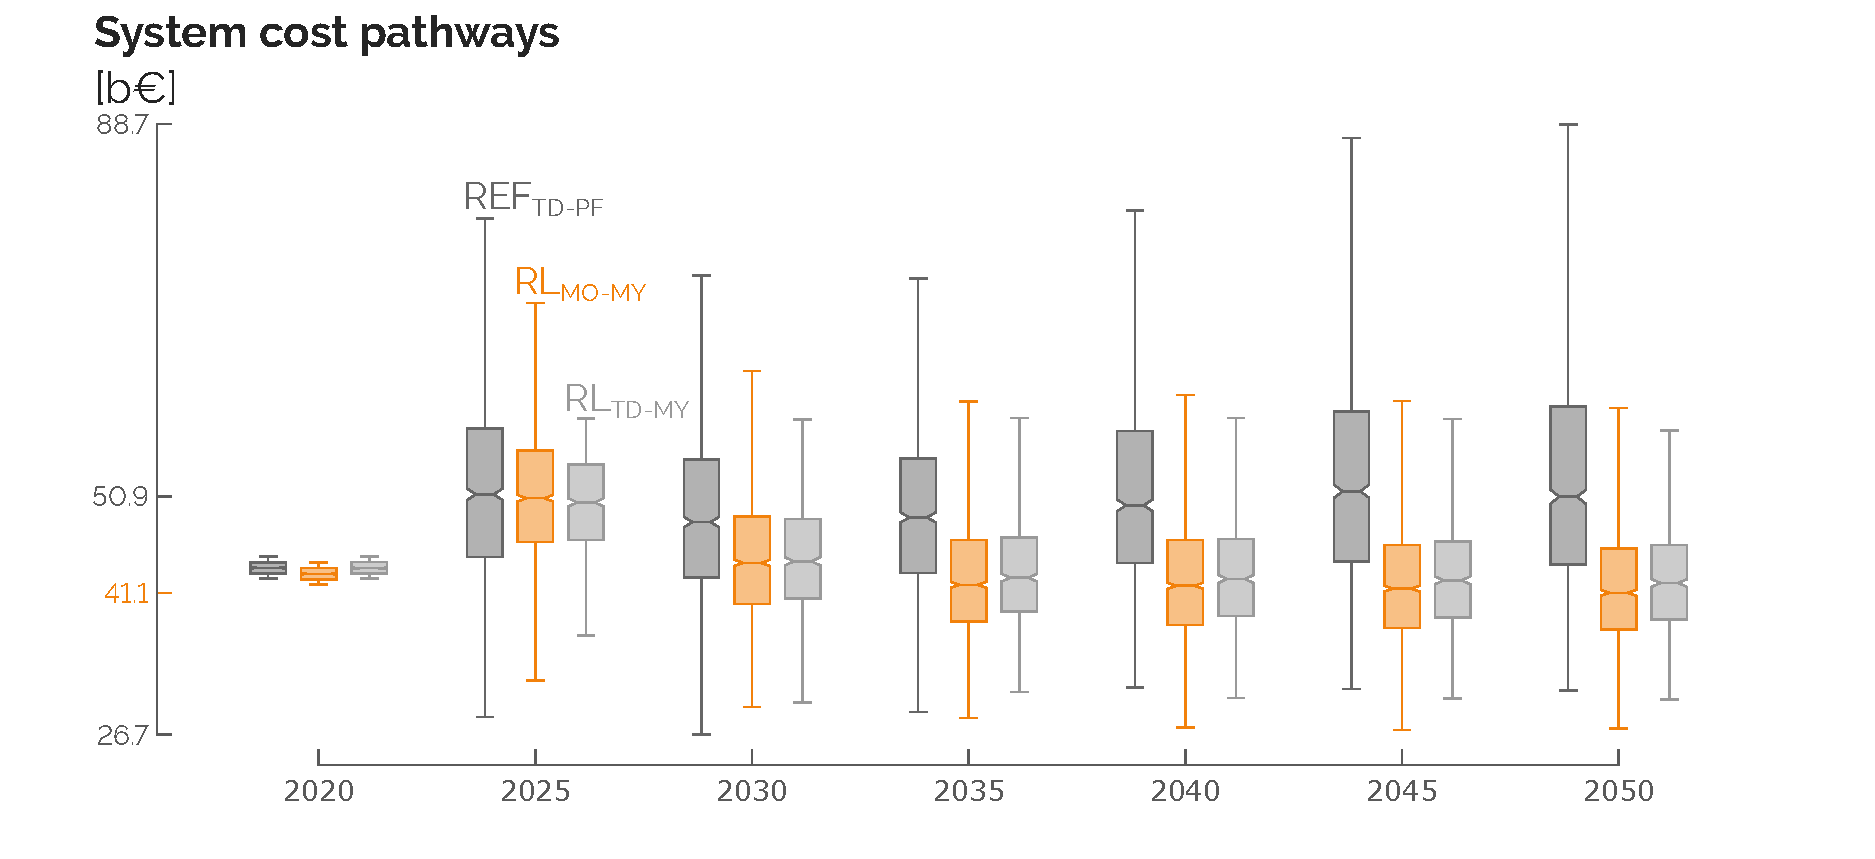
\includegraphics[width=0.8\textwidth]{System_cost_pathway.pdf}
\caption{Comparison of annual system costs pathways from the perfect foresight optimisation under uncertainties ($\text{REF}_{\text{TD-PF}}$), the \gls{RL}-based myopic optimisation on the monthly ($\text{RL}_{\text{MO-MY}}$) and hourly ($\text{RL}_{\text{TD-MY}}$) models.}
\label{fig:System_cost_pathway}
\end{figure}

The analysis of the cumulative costs shows that the \gls{OPEX} is the main difference between myopic and perfect foresight transitions (see Figure \ref{fig:Opex_Capex_Salvage_comp}). Successful myopic transitions have a lower \gls{OPEX} thanks to the agent's actions and importing more electrofuels, especially e-ammonia that is more imported in the myopic optimisation to supply \gls{CCGT} in case \gls{SMR} is not available.

We observe also similar distributions between the monthly and hourly myopic results that confirm the good approximation provided by the monthly approach.

\begin{figure}[!htbp]
\centering
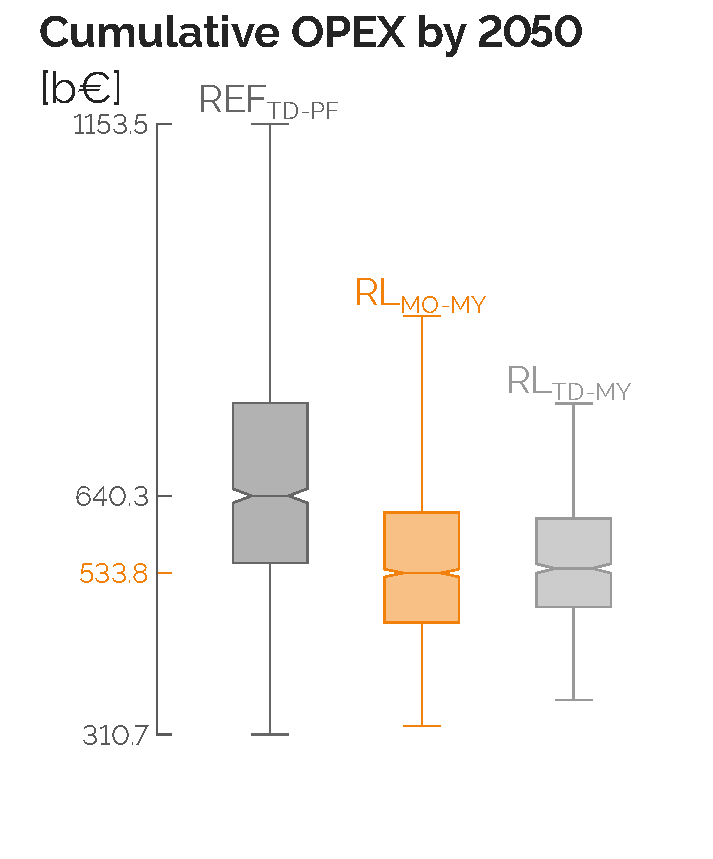
\includegraphics[width=0.325\textwidth]{Opex_2050_comp.pdf}
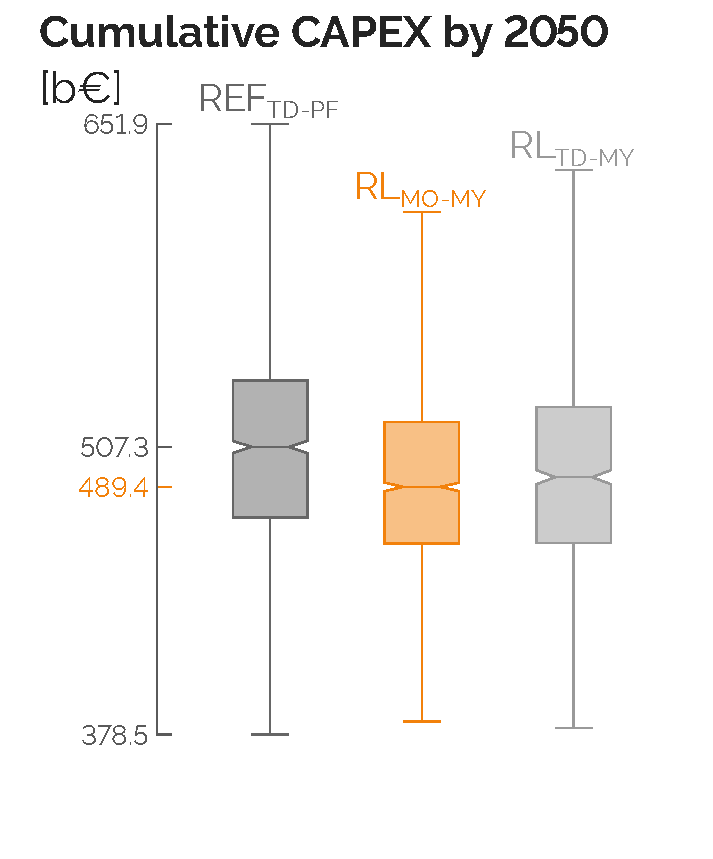
\includegraphics[width=0.325\textwidth]{Capex_2050_comp.pdf}
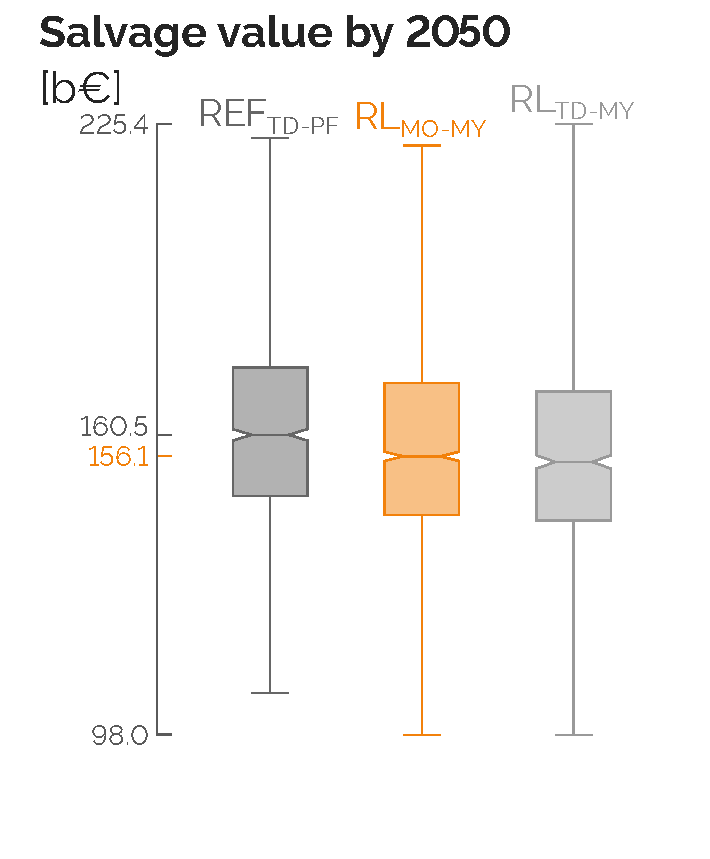
\includegraphics[width=0.325\textwidth]{Salvage_2050_comp.pdf}
\caption{Comparison of cumulative OPEX (top-left), CAPEX (top-right) and salvage value (bottom) in 2050 from the perfect foresight optimisation under uncertainties ($\text{REF}_{\text{TD-PF}}$), the \gls{RL}-based myopic optimisation on the monthly ($\text{RL}_{\text{MO-MY}}$) and hourly ($\text{RL}_{\text{TD-MY}}$) models.}
\label{fig:Opex_Capex_Salvage_comp}
\end{figure}

\section{Conclusions}
\label{sec:RL:conclusions}
In the literature, two options are investigated to explore transition pathways of a whole-energy system. On the one hand, in perfect foresight optimisation, a full knowledge of the parameters is assumed over the entire time horizon. On the other hand, myopic optimisation considers a sequence of more limited time windows leading to the end of the time horizon, to add more realism \cite{poncelet2016myopic}. To meet objective of climate change mitigation, this case requires a prescribed \ce{CO2}-trajectory \cite{fais2016impact}. However, since the effect of \ce{CO2}-emissions in climate change is cumulative, the total amount of these emissions matters more than the trajectory itself. Consequently, we have applied the \acrfull{RL} approach on the environment of the Belgian myopic pathway optimisation under uncertainties.

In \gls{RL} framework, the agent had four actions to support the 2020-2050 transition: (i) limiting the \ce{CO2}-emissions at the end of each successive time window and limiting the consumption of (ii) fossil gas, (iii) \acrfull{LFO} and (iv) coal. The reward fed back by the environment to the agent focused first on meeting the \ce{CO2}-budget, 1.2\,Gt\ce{CO2} equivalent to 10 years at the current level of emissions. A secondary focus is also put on aiming at minimum transition cost. To know its progress through the transition, the agent had the information of the cumulative emissions and costs as well the share of renewable energy carriers in the primary energy mix and the system overall efficiency.

This \gls{RL}-based exploration pointed out that short-term actions were needed to hope succeeding such a transition, as also demonstrated by \citet{luderer2018residual}. Where \gls{LFO} becomes less cost-competitive in the near-future, limiting the use of coal should be done at any cost. Then, fossil gas should be replaced by e-methane in the mid-term while limiting the overall emissions becomes more effective by the end of the transition. The analysis of the share of renewables in the primary energy mix highlighted intermediate milestones to have higher chances to succeed the transition. Below 54\% of renewables in the mix in the near-future, these chances become much more limited, \ie the no-go zone. 

Finally, we have compared the results coming from this \gls{RL}-based myopic optimisation with monthly time-resolution with the hourly perfect foresight approach. These myopic optimisations provided pathways respecting the \ce{CO2}-budget that were more drastic in cutting emissions in the short-term than the perfect. Supported by the agent's actions, we could reach cheaper energy system than what the perfect foresight could give. With the advantage of the smaller computational burden, the monthly model myopic model was also found to be a good proxy with its equivalent based on hourly time-resolution.

In conclusion, via the application of the \gls{RL} approach, we have widely explored the different myopic transition pathways and identified sweet-spots (and no-go zones) to succeed a transition with an ambitious \ce{CO2}-budget target. It also highlighted the actions to take to effectively support a whole-energy system transition.